%%%%%%%%%%%%%%%%%%%%%%%%%%%%%%%%%%%%%%%%%%%%%%%%%
%%%
%%% Auteur : Stéphane Péchard - stephane.pechard@univ-nantes.fr
%%% Fichier : 4-metriques.tex - chapitre 4 :  Critères objectifs de qualité vidéo et création d'une base de séquences (30 pages)
%%% Version : 0.1
%%% Date : 2007/09/10
%%%
%%%%%%%%%%%%%%%%%%%%%%%%%%%%%%%%%%%%%%%%%%%%%%%%%
\chapter{Critères objectifs de qualité vidéo : état de l'art} \label{chap:criteres}
\opt{final}{\lettrine[lines=4]{L}{a littérature propose}}\opt{nofinal}{La littérature propose} de nombreuses méthodes d'évaluation objective de la qualité de la vidéo. Ce chapitre a pour objectif de présenter de façon structurée une vue d'ensemble des principales approches existantes. Nous la limitons sciemment au domaine applicatif qui nous concerne : le codage. Pourtant, les applications de l'évaluation objective de la qualité vidéo sont plus diverses. La transmission, les post-traitements, les capteurs ou les afficheurs sont également des éléments pouvant faire l'objet de critères de qualité spécifiques. Les critères objectifs de qualité vidéo sont de trois types différents, suivant la disponibilité ou non du signal vidéo d'origine, dit de référence, car supposé non dégradé. Pour le premier type, appelé avec référence complète (noté FR pour \emph{Full Reference}), les méthodes disposent de la vidéo de référence en plus de la vidéo dont la qualité est à mesurer. Ceci est le cas ici car le codage s'effectue à partir de la vidéo de référence et la version dégradée est la vidéo après codage/décodage. La plupart des méthodes proposées dans la littérature fonctionnent de cette manière et c'est ce type que nous traiterons ici en grande majorité. Nous ne considérerons pas le cas du transcodage. Le second type de méthodes, appelées avec référence réduite (RR pour \emph{Reduced Reference}), produit une mesure de qualité en ne disposant que d'un ensemble réduit de caractéristiques mesurées sur la référence. Les mêmes caractéristiques calculées sur la vidéo dégradée leur sont comparées afin de construire la note de qualité finale. Le peu d'information disponible pour la conception rend celle-ci plus difficile que pour les méthodes avec référence complète. Par contre, ce type de méthode s'applique très bien à la transmission de la vidéo car la référence réduite est codée avec une quantité d'informations binaires très réduite par rapport à celle utilisée dans le codage du contenu. Enfin, les méthodes sans référence (notées NR pour \emph{No Reference}) calculent un critère sans aucune connaissance du signal d'origine. Alors que l'\oe il humain est le plus souvent capable d'évaluer une qualité d'image sans connaitre la référence associée, la conception d'un critère de qualité visuelle sans référence est une tâche particulièrement complexe. C'est pourquoi peu de critères de ce type ont été proposés dans la littérature jusqu'à présent. Cependant, pour améliorer les performances des méthodes avec référence réduite ou sans références, il est possible de s'appuyer des a priori sur le système dégradant utilisé.

Nous utiliserons en plus ici une classification de plus haut niveau que celle distinguant les niveaux de disponibilité de la référence. Celle que nous adoptons distingue les approches n'exploitant pas les propriétés du système visuel humain de celles qui en exploitent. Les premières tiennent uniquement compte des données brutes de la vidéo. Les secondes intègrent des principes de plus ou moins haut niveau du système visuel humain. Ceci leur permet de rendre compte de l'impact des données sur la perception de la qualité. Dans cette catégorie d'approche, plusieurs courants co-existent. La figure~\ref{fig:vueGlobale} tente de représenter l'ensemble des approches abordées dans ce chapitre, avec des exemples de critères pour chacune d'elle. Ces critères seront mentionnés et détaillés dans la suite de ce chapitre.

\begin{figure}[htbp]
  \centering
  \begin{tikzpicture}[text centered,scale=1.04]% \begin{tikzpicture}[text centered]

% ellipses bleues
\filldraw[thick,dashed,fill=blue!20] (1.5,0.1) ellipse (3cm and 1.2cm);
\filldraw[thick,dashed,fill=blue!20] (-0.5,-1.75) ellipse (2cm and 0.7cm);
\filldraw[thick,dashed,fill=blue!20] (1,-3.5) ellipse (3cm and 1cm);
\filldraw[thick,dashed,fill=blue!20] (6.5,-1.5) ellipse (2.5cm and 2cm);

% ellipses
\draw (-2,-1.5) ellipse (3cm and 2cm);
\draw (3,-1.5) ellipse (6cm and 3cm);

% texte
\draw (-4,0.75) node[text width=2cm] {\strong{Approches signal}};
\draw (7.5,-4.5) node[text width=3cm] {\strong{Approches perceptuelles}};

\draw (-4,-1.5) node[text width=2cm] {PSNR WPSNR};
\draw (-2,-0.5) node {VQM};

\draw (2.8,0.25) node[text width=4cm,color=blue!80] {\strong{Modèles avec connaissance du système dégradant}};
\draw (1,1) node {Farias};
\draw (0,0.5) node {NROQM};
\draw (0,-0.25) node {Marziliano};
\draw (0.8,-0.8) node {Wang};

\draw (1.75,-3.75) node[text width=4cm,color=blue!80] {\strong{Modèles basés sur des principes perceptuels}};
\draw (-1.25,-3.2) node {NHK};
\draw (-0.5,-2.9) node {KPN};
\draw (1.5,-2.9) node {Tapestries};

\draw (0,-1.75) node[color=blue!80,text width=2cm] {\strong{Modèles structurels}};
\draw (-1.5,-2) node {SSIM};
\draw (-1.5,-1.5) node {VSNR};

\draw (6.5,-0.5) node[text width=3cm,color=blue!80] {\strong{Modèles basés sur le SVH bas niveau}};
\draw (8,-1.5) node {Sarnoff};
\draw (7.5,-2.25) node {NVFM};
\draw (6.5,-3) node {VDP};
\draw (5.5,-2.25) node {PDM};
\draw (5,-1.5) node {DVQ};

% \end{tikzpicture}
\end{tikzpicture}
  \caption{Vue d'ensemble des critères objectifs de qualité vidéo.}
  \label{fig:vueGlobale}
\end{figure}

Dans la catégorie des approches perceptuelles, nous distinguons trois groupes d'approche. Le premier est composé des approches basées sur la modélisation de la vision humaine bas niveau. Le second correspond aux approches basées sur la fidélité structurelle. Celles-ci incluent des propriétés de plus haut niveau du système visuel humain. Le dernier groupe est composé des approches basées sur la mesure explicite de dégradations haut niveau.

Ce chapitre est organisé de la manière suivante. Nous commencerons par développer les critères objectifs basés signal. Nous délimiterons leur usage, tout en nuançant les critiques portées habituellement à leur égard. Les sections suivantes traiteront successivement des approches basées sur la modélisation fine de la vision humaine bas niveau, des approches basées sur la fidélité structurelle et des approches basées sur la mesure explicite de dégradations haut niveau. Nous terminerons par une discussion sur les différentes questions soulevées par ces approches.


\section{Défauts\dots mais aussi mérites du PSNR} \label{sec:modelesMathematiques}
Les communautés scientifiques du codage et du traitement de l'image et de la vidéo utilisent depuis longtemps des métriques basées signal. Il s'agit du rapport signal sur bruit crête, ou PSNR \emph{(Peak signal to noise ratio)} et de ses dérivés. Cet usage est devenu presque exclusif, entretenant l'habitude de leur manipulation. Il y a plusieurs raisons à cet usage. La principale est que le PSNR n'est pas systématiquement inadapté. Il existe des situations où son utilisation a du sens. La seconde raison est sa simplicité et sa rapidité d'exécution, qui le rend d'utilisation très aisée. Enfin jusqu'ici, peu d'autres métriques objectives de la littérature sont venues remettre cet usage en question.

Cependant, la communauté de la qualité d'image et de la vidéo s'interroge sur le bien fondé d'une telle popularité~\cite{girod-mse, eskicioglu-icassp2000, vqeg-frtv2}. S'il est en effet critiquable et facilement mis en défaut, il convient pourtant de lui reconnaitre quelques vertus. Après tout, il ne serait tout simplement pas utilisé s'il ne rendait pas un minimum de service aux utilisateurs. C'est d'ailleurs une critique plus générale qu'il faut énoncer. Le bon usage d'une métrique passe par la maitrise de ses capacités et de ses limites. La métrique idéale et universelle n'existe pas encore. Revenons maintenant sur les critiques usuelles portées à l'encontre du PSNR avant de nuancer notre propos par quelques exemples.


\subsection{Les critiques habituelles}
Le défaut majeur imputable au PSNR est que son calcul étant effectué pixel par pixel, tous ayant la même importance, il ne tient pas compte de l'activité du contenu de la vidéo. Cela a deux conséquences. La première est qu'un désalignement spatial ou temporel a des effets particulièrement désastreux sur la mesure. Alors que le décalage d'une image d'un pixel est généralement imperceptible pour l'observateur, le PSNR le considérera comme une dégradation non négligeable. De même, une désynchronisation temporelle sera particulièrement mal évaluée. C'est pour cela qu'il est incapable de prédire l'impact des erreurs de transmission. La seconde conséquence est que le cumul des erreurs tel qu'il est effectué n'a aucune considération perceptuelle de ces erreurs. Il ne permet pas d'établir une relation forte et cohérente avec les notes de qualité vidéo fournies par l'observateur moyen. À titre d'exemple, nous avons calculé les performances du PSNR sur l'ensemble de 168 séquences dégradées de la base présentée à l'annexe~\ref{annex:base}. Si nous calculons le coefficient de corrélation entre les évaluations subjectives fournies par les observateurs et le PSNR, nous obtenons une très faible valeur de 0,4077. La figure~\ref{fig:nuagePSNRlcd} présente les MOS prédits par le PSNR en fonction des mesures subjectives mesurés sur écran LCD.

\begin{figure}[htbp]
	\centering
	\begin{tikzpicture}[only marks, scale=0.07]
	\pgfsetplotmarksize{1cm}
	\draw plot[mark=+] file {plot/chap4/MOSLCD-MOSpPSNR.txt};
	\draw[->] (0,0) -- coordinate (x axis) (85,0);
	\draw[->] (0,0) -- coordinate (y axis) (0,85);
	\foreach \x in {0,20,40,60,80} \draw (\x cm,1cm) -- (\x cm,-1cm) node[anchor=north] {\x};
	\foreach \y in {0,20,40,60,80} \draw (1cm,\y cm) -- (-1cm,\y cm) node[anchor=east] {\y};
	\node[below=0.5cm] at (x axis) {MOS prédits};
	\node[left=0.9cm,rotate=90] at (0,50) {MOS};
	\draw[dotted] (0,0) -- (80,80);
	\end{tikzpicture}
	\caption{MOS prédits par le PSNR en fonction des MOS subjectifs mesurés sur écran LCD.}
	\label{fig:nuagePSNRlcd}
\end{figure}

La conséquence de ces défauts est un manque de cohérence et de robustesse. Le PSNR n'est pas capable de bien prédire la qualité entre différents contenus, différentes résolutions, différentes cadence d'affichage ou différents systèmes dégradants. Illustrons cela par un exemple. Les figures~\ref{fig:PSNR1},~\ref{fig:PSNR2} et~\ref{fig:PSNR3} présentent le MOS en fonction du PSNR pour trois contenus différents de la base de l'annexe~\ref{annex:base}. Ces trois mêmes courbes sont regroupées sur la figure~\ref{fig:PSNR123}. Nous constatons qu'avec un même contenu et un même système dégradant, la relation entre le PSNR et le MOS est globalement monotone, même si pour certains contenus tels que \emph{Voile}, nous observons une non monotonie. La figure~\ref{fig:PSNR123} illustre parfaitement le manque de robustesse inter-contenu du PSNR. Les valeurs maximales des MOS des trois contenus sont de 69,1, 68,3 et 67,3, c'est-à-dire très proches compte tenu de la dynamique de l'échelle. En revanche, les PSNR correspondant sont respectivement de 27,16 dB, 33,61 dB et 40,2 dB. Cette différence est indiquée d'une flèche sur la figure~\ref{fig:PSNR123}. Le même type de problème survient si le PSNR est utilisé pour évaluer différents types de dégradations~\cite{ebrahimi-spie2004}. Il est donc impossible de comparer des PSNR calculés dans des scénarii trop différents, comme par exemple dans l'évaluation de performances de différents codeurs.

\begin{figure}[htbp]
	\centering
	\subfloat[\label{fig:PSNR1} Séquence \emph{Parkrun}.]{\includegraphics[width=0.48\linewidth, trim=80 25 110 82, page = 1]{plot/MOS-PSNR}}\hfill
	\subfloat[\label{fig:PSNR2} Séquence \emph{Duck Fly}.]{\includegraphics[width=0.48\linewidth, trim=80 25 110 82, page = 2]{plot/MOS-PSNR}}\\
	\subfloat[\label{fig:PSNR3} Séquence \emph{Voile}.]{\includegraphics[width=0.48\linewidth, trim=80 25 110 82, page = 3]{plot/MOS-PSNR}}\hfill
	\subfloat[\label{fig:PSNR123} Séquences \emph{Parkrun}, \emph{Duck Fly} et \emph{Voile}.]{\includegraphics[width=0.48\linewidth, trim=80 25 110 82, page = 4]{plot/MOS-PSNR}}\\
	\caption{MOS en fonction du PSNR (en dB) pour trois séquences différentes.}
\end{figure}

Cela étant, ces défauts ne sont pas systématiquement comblés par les autres critères de la littérature. En fait, peu s'avèrent réellement robustes dans toutes les situations. C'est pourquoi elles sont généralement spécialisées, comme peut l'être le PSNR, mais dans une moindre mesure.


\subsection{Application à un contexte limité}
L'exemple précédent délimite des conditions d'utilisation du PSNR. S'il est restreint à un contexte donné, il peut fournir une relation forte avec les MOS.  Rodrigues~\cite{rodrigues-pcs2007} l'utilise pour évaluer sa technique d'amélioration du codage MPEG-4 de l'erreur de prédiction du mouvement des images B. Il compare le PSNR moyen des images codées en mode B d'une séquence avec et sans l'usage de cette technique. Il effectue cette comparaison sur plusieurs contenus, mais il ne compare pas les PSNR d'un contenu à l'autre. De même, il calcule le PSNR sur les trois composantes couleurs pour mesurer le gain obtenu sur chacune d'elle, mais il ne compare pas les PSNR entre différentes composantes.

Les limites du PSNR sont, en l'occurence, bien prises en compte par Rodrigues. Son usage doit ainsi se limiter à des comparaisons où peu de conditions changent. Par exemple, le PSNR peut être utilisé pour mesurer le gain en débit obtenu par des algorithmes centrés sur une très petite partie d'un schéma de codage~\cite{merkle-eusipco2007}. À l'inverse, une régulation de débit basée sur le PSNR peut poser des problèmes, car aucun contrôle sur la qualité visuelle n'est alors effectué.


\subsection{Le PSNR amélioré}
Il existe quelques tentatives d'amélioration du PSNR, notamment le WSNR \emph{(Weighted signal to noise ratio)}~\cite{damera-ieee2000}. Cela consiste à appliquer une pondération du SNR par une CSF comme celle de Mannos et Sakrison~\cite{mannos-ieee1974}. Le calcul de l'erreur locale est ainsi plus pertinente, mais le problème du cumul n'est pas traité. Cette méthode permet de gagner en précision par rapport au SNR, mais sans atteindre les performances d'autres critères.

Oelbaum~\cite{oelbaum-pcs2007} propose une technique d'amélioration des critères de qualité en général et applicable entre autre au PSNR. Elle est basée sur l'observation que nous venons de faire : la corrélation entre les MOS et les notes objectives est forte dans le cas du codage à plusieurs débits d'un même contenu donné par un codeur donné. L'auteur exploite cette propriété pour réduire la différence entre la qualité prédite et la qualité subjective. La figure~\ref{fig:methodOelbaum} présente son modèle. La méthode nécessite la création de deux séquences additionnelles codées/décodées. La première doit être de haute qualité visuelle, entre 80 et 100 sur une échelle de 0 à 100. La seconde doit être de basse qualité, entre 0 et 20. Pour déterminer ces qualités, il faut donc effectuer des tests subjectifs. L'application de la méthode au PSNR est la suivante. Fixons les qualités subjectives des ancres de haute et basse qualité à 90 et 10 respectivement. Leurs PSNR sont $\mathit{PSNR}_h$ et $\mathit{PSNR}_b$ respectivement. Deux paramètres $\mathit{slope}$ et $\mathit{offset}$ sont calculés de la manière suivante :
\begin{equation}
\mathit{slope}=\frac{\mathit{PSNR}_h - \mathit{PSNR}_b}{90-10}\qquad \text{et}\qquad \mathit{offset} = \mathit{PSNR}_b - (10\times \mathit{slope}).
\end{equation}
%
Une fois ces paramètres connus, le PSNR amélioré d'une séquence dégradée, appelé PSNR$^+$, est calculé par :
\begin{equation}
\mathit{PSNR}^+ = \frac{\mathit{PSNR} - \mathit{offset}}{\mathit{slope}}
\end{equation}

\begin{figure}[htbp]
	\centering
	\begin{tikzpicture}[text centered, node distance = 3cm]% \begin{tikzpicture}[text centered, node distance = 3cm]
% Place nodes
	\node[text width=1.5cm] (ref) {séquence originale};
	\node[action, right of=ref, node distance = 2.2cm] (codage) {codage};
	\node[right of=codage, text width=2cm, node distance = 2.5cm] (deg) {séquence dégradée};
	\node[below of=deg, node distance = 2cm, text width=2cm, node distance = 2.5cm] (seqBas) {séquence de basse qualité};
	\node[below of=seqBas, node distance = 2cm, text width=2cm, node distance = 2.5cm] (seqHaut) {séquence de haute qualité};
	\node[action, right of=deg, text width=1.5cm] (critDeg) {critère de qualité};
	\node[action, right of=seqBas, text width=1.5cm] (critBas) {critère de qualité};
	\node[action, right of=seqHaut, text width=1.5cm] (critHaut) {critère de qualité};
	\node[below of=critBas, node distance = 1cm] (tmp) {};
	\node[action, right of=tmp, text width=3cm, rotate=90, node distance = 3.2cm] (regression) {régression};
	\node[action, right of=critDeg, node distance = 3.2cm] (correction) {correction};
	\node[right of=correction, node distance = 2cm] (psnr) {$\mathit{PSNR}^+$};

% Draw edges
	\path[fleche] (ref) -- (codage);
	\path[fleche] (codage) -- (deg);
	\path[fleche] (deg) -- (critDeg);
	\path[fleche] (codage) |- (seqBas);
	\path[fleche] (seqBas) -- (critBas);
	\path[fleche] (codage) |- (seqHaut);
	\path[fleche] (seqHaut) -- (critHaut);
	\path[fleche] (critBas) -- (regression) node[above=2pt,pos=0.5] {$\mathit{PSNR}_b$};
	\path[fleche] (critHaut) -- (regression) node[below=4pt,pos=0.5] {$\mathit{PSNR}_h$};
	\path[fleche] (critDeg) -- (correction) node[above,pos=0.5] {PSNR};
	\path[fleche] (regression) -- (correction) node[right,pos=0.5] {$\mathit{slope, offset}$};
	\path[fleche] (correction) -- (psnr);
% \end{tikzpicture}
\end{tikzpicture}
	\caption{Schéma de la technique d'amélioration des critères de qualité d'Oelbaum~\cite{oelbaum-pcs2007}.}
	\label{fig:methodOelbaum}
\end{figure}

L'auteur évalue les performances de sa méthode sur un ensemble de 54 séquences CIF dégradées par un codage H.264 et évaluées par 20 observateurs. Il ne précise pas les paramètres de codage de ces séquences. Les ancres basse et haute sont codées par le codeur de référence H.264~\cite{h264-jm} en fixant les pas de quantification pour chacune. L'auteur ne précise pas non plus si les performances qu'il fournit sont calculées après l'application d'une fonction d'ajustement. Une telle fonction permet de transformer les PSNR$^+$ en une prédiction du MOS, appelé MOSp. Le coefficient de corrélation entre les MOS et les PSNR$^+$ est de 0,831 alors qu'il est de 0,665 avec un simple PSNR. L'\emph{outlier ratio} des PSNR$^+$ est de 0,722, alors qu'il est de 0,907 pour les PSNR. Cet indicateur calcule le rapport $\frac{N_{e}}{N_n}$ entre le nombre de configurations mal évaluées $N_e$ et le nombre total de notes objectives $N_n$. Une configuration est considérée comme mal évaluée si $|\MOS - \MOSp| > 2\times\IC$ avec $\IC$ l'intervalle de confiance à 95\% du MOS. Le gain est significatif, sans pour autant suffire à rendre le PSNR très robuste.

Outre ce gain en performance insuffisant dans le cas du PSNR, cette approche originale a d'autres désavantages. Le premier est qu'elle nécessite la création de nouvelles séquences, dont il faut évaluer la qualité de manière subjective pour que la régression linéaire soit efficace. Cela peut être fait par des experts sans mettre en place un ensemble de tests psychophysiques mais nécessite tout de même une intervention, ce qui réduit l'automatisation de la méthode. De plus, pour créer ces ancres basse et haute, l'auteur conseille d'utiliser un codeur proche, en termes de technologie, de celui utilisé pour coder les séquences évaluées. Enfin, dans le cas plus général de l'utilisation de cette méthode avec des critères de qualité vidéo sans référence, elle nécessite tout de même les paramètres $\mathit{slope}$ et $\mathit{offset}$. En conséquence, un critère sans référence devient avec référence réduite, celle-ci étant constituée de ces deux paramètres.


\section{Approches basées sur la modélisation fine de la vision humaine bas niveau}
Ce type d'approche cherche à modéliser plus ou moins finement les phénomènes bas niveau de la vision. Les connaissances nécessaires à cette modélisation sont le plus souvent issus d'expérimentations psychovisuelles. La complexité du système de vision humaine fait que ces travaux durent depuis de nombreuses années. Les premiers résultats portaient sur l'image fixe, avant de s'intéresser plus récemment à la vidéo.


\subsection{Métriques de qualité en images fixes}
Le schéma classique de la version la plus évoluée d'une telle métrique est donné sur la figure~\ref{fig:ApprocheSVH}. Historiquement, les différents éléments qui le constitue sont apparus progressivement.

\begin{figure}[htbp]
	\centering
	\begin{tikzpicture}[text centered, node distance = 3cm]% \begin{tikzpicture}[text centered]
% Place nodes
	\node[text width=2cm] (ref) {séquence originale};
	\node[action, below of=ref, text width=2.5cm, node distance = 2.4cm] (couleur) {décomposition dans un espace de couleurs antagonistes};
	\node[below of=couleur, text width=2cm, node distance = 2.4cm] (deg) {séquence dégradée};
	\node[action, right of=couleur, text width=2cm] (csf) {fonction de sensibilité aux contrastes};
	\node[action, right of=csf, text width=2.5cm] (canaux) {décomposition en canaux perceptuels};
	\node[action, right of=canaux, text width=2cm] (masq) {fonction de masquage};
	\node[action, right of=masq, node distance = 2cm] (cumul) {cumul};
	\node[right of=cumul, node distance = 1.5cm] (note) {note};

% Draw edges
	\path[fleche] (ref) -- (couleur);
	\path[fleche] (deg) -- (couleur);
	\path[fleche] (couleur) -- (csf);
	\path[fleche] (csf) -- (canaux);
	\path[fleche] (canaux) -- (masq);
	\path[fleche] (masq) -- (cumul);
	\path[fleche] (cumul) -- (note);
% \end{tikzpicture}\end{tikzpicture}
	\caption{Schéma générique d'une métrique de qualité basée sur la modélisation fine de la vision humaine bas niveau.}
	\label{fig:ApprocheSVH}
\end{figure}

Les premières modélisations du système visuel humain reposent sur une approche à un seul canal perceptuel. Dans les travaux de Mannos, seule une fonction de sensibilité aux contrastes (CSF) permet de définir le système~\cite{mannos-ieee1974}. Une CSF décrit l'évolution de la sensibilité visuelle en fonction des fréquences spatiales et de l'orientation du signal à détecter. La sensibilité visuelle est définie comme l'inverse du contraste d'un signal à son seuil différentiel de visibilité.

Un élément important de la perception est l'effet de masquage. Celui-ci se caractérise par la modification de la perception d'un signal par la présence d'un autre signal. En pratique, cela consiste à prendre en considération le contexte spatial et temporel dans le calcul d'une mesure locale comme un contraste. L'inclusion de ces effets de masquage dans les métriques de qualité mono-canal a permis de sensiblement les améliorer~\cite{kusayama-pcs2001}.

Les effets de masquage sont mieux caractériser par les modélisations multi-canaux que par les modélisations mono-canal car ils permettent d’intégrer certaines spécificités des champs récepteurs du système visuel. Zetzsche~\cite{zetzsche-vcip1989} propose le premier modèle utilisant une décomposition en canaux perceptuels. Celle-ci utilise une pyramide ROG \emph{(ratio of gaussian)} à cinq niveaux de résolution et un ensemble de filtres gaboriens ayant une sélectivité angulaire de 30 degrés. Plusieurs types de décomposition ont été proposés. Par exemple, le VDP de Daly~\cite{daly-vdp} utilise une version adaptée de la transformée Cortex de Watson~\cite{watson-cortex}. Celle-ci se caractérise par des filtres à sélectivité radiale dyadique et à sélectivité angulaire de 30 degrés. Lubin~\cite{lubin-jnd} décompose les images originales et dégradées en sous-bandes à l'aide de sept filtres passe-bandes de fréquences centrales allant de 32 à 0,5 cycle par degré. Une décomposition pyramidale à cinq niveaux permet ensuite de créer un ensemble d'images de plusieurs résolutions.

Le premier critère de qualité d'images en couleur a été proposé par Faugeras~\cite{faugeras-ieee1979}. À partir de la réponse des cônes de la rétine, il effectue une décomposition dans un espace couleur perceptuel. Il obtient ainsi une composante achromatique et deux composantes chromatiques. Ce calcul repose sur la théorie classique des signaux antagonistes, largement utilisé~\cite{lambrecht-cmpqm,lai-perceptual,krauskopf-vr1982}. L'\oe il humain étant plus sensible à la luminance qu'à la chrominance, il est courant de donner moins d'importance ou de précision à cette dernière. C'est par exemple le cas de la décomposition en canaux de Le Callet~\cite{lecallet-phd} qui limite le plan fréquentiel des composantes chromatiques aux deux premières bandes de fréquences spatiales, alors que celui de la composante achromatique en compte quatre. De même, le cumul inter-composante exploite cette propriété en privilégiant la luminance.

La dernière étape de cumul est très importante dans la mesure où elle permet d'obtenir la note de qualité finale à partir des contributions locales. Cependant, ce cumul est souvent simplifié car la manière dont il est opéré par le système visuel humain n'est toujours pas bien connue~\cite{wang-ovqa}. Peu d'originalité en découle, les auteurs préférant privilégier les étages précédents. La sommation de Minkowski est alors souvent utilisée pour intégrer les mesures locales. Cette sommation est de la forme :
\begin{equation}
S_M = \left( \frac{1}{N_v} \sum\limits_{i=1}^{N_v} v_i^\beta \right)^{\frac{1}{\beta}}
\end{equation}
%
avec $\beta$ l'exposant de la sommation et $v$ le vecteur de $N_v$ éléments. Cependant, cette somme ne permet de pondérer les données qu’en fonction de leur amplitude et non en fonction de leur répartition spatiale ou temporelle~\cite{wang-icassp2002}. La complexité des phénomènes haut niveau mis en jeu lors de la construction finale de la note subjective de qualité n'est donc pas entièrement considérée.


\subsection{Passage à la vidéo}
La conception de critères objectifs de qualité adaptés à la vidéo pose l'épineux problème de la dimension temporelle. Celle-ci implique des modifications à la fois au niveau du calcul des erreurs locales et de leur cumul en une note de qualité. Ce type de métrique de qualité vidéo peut ainsi se décomposer en deux étages principaux comme le montre la figure~\ref{fig:ApprocheSVHVideo}.

\begin{figure}[htbp]
	\centering
	\begin{tikzpicture}[text centered, node distance = 3cm]% \begin{tikzpicture}[text centered]
% Place nodes
	\node[text width=2cm] (ref) {séquence originale};
	\node[action, right of=ref, text width=3cm, node distance = 3.5cm] (mesure) {mesure des erreurs locales};
	\node[action, right of=mesure] (cumul) {cumul};
	\node[right of=cumul, node distance = 2cm] (note) {note};

% Draw edges
	\path[fleche] (ref) -- (mesure);
	\path[fleche] (mesure) -- (cumul);
	\path[fleche] (cumul) -- (note);
% \end{tikzpicture}\end{tikzpicture}
	\caption{Les deux étages principaux d'un critère de qualité vidéo.}
	\label{fig:ApprocheSVHVideo}
\end{figure}

Il est courant que les critères d'évaluation de la qualité vidéo soient adaptés de critères pour images fixes. Ainsi, Watson adapte sa DCTune~\cite{watson-dctune} pour proposer la DVQ~\cite{watson-dvq}. Les éléments de vision qu'il intègre sont assez nombreux : adaptation en luminance, décomposition en composantes couleur, décomposition spatio-fréquentielle, filtrage spatial et temporel et masquage de contraste. Le point intéressant est le passage de la notion de visibilité de bruit DCT de l'image à la vidéo. L'auteur intègre pour cela un modèle mathématique qui s'adapte aux seuils de visibilité pour rendre compte du mouvement. Ce modèle établit un seuil pour chaque fonction DCT de base 8\texttimes8. Les paramètres mathématiques ont été déterminés par des simulations de stimuli de bruit DCT dynamique. À partir d'expériences psychophysiques, Watson propose un modèle tridimensionnel séparable, produit d'une fonction temporelle, d'une fonction spatiale et d'une fonction d'orientation. Le cumul final est effectué par une sommation de Minkowski.

Le premier modèle de vision connu est celui de Lukas et Budrikis~\cite{lukas-PQMonVM}, adaptée à la télévision noir et blanc. Il incorpore deux éléments principaux. Le premier est un modèle spatio-temporel non linéaire permettant de filtrer les erreurs de la séquence dégradée. La non linéarité agit comme un contrôle du gain, permettant au modèle de s'adapter aux changements de niveau de luminance de fond. Le second élément est une fonction de masquage. Le stimulus d'entrée est pondéré suivant la quantité d'activité spatio-temporelle locale. Enfin, la mesure de distorsion est calculée par la norme $L_p$ de l'image des erreurs masquées. Les auteurs montrent que les observateurs basent leur jugement sur l'évaluation de zones critiques plutôt que sur l'ensemble de la séquence. Ils justifient ainsi la pertinence de la mesure d'erreurs locales. Cependant, le cumul appliqué à ces erreurs est une simple moyenne, ce qui ne rend le résultat final beaucoup moins pertinent.

Plus récemment, Winkler a proposé la PDM \emph{(Perceptual distortion metric)}~\cite{winkler-hvei1999} pour l’évaluation de qualité de séquences d’images couleur. Il s'agit d'une amélioration de la NVFM \emph{(Normalized video fidelity metric)} de Lambrecht~\cite{lindh-icip1996}. Après la décomposition des composantes couleur, la décomposition perceptuelle est effectuée dans le temps, puis dans l'espace. L'aspect temporel est considéré comme décomposable par un filtre passe-bas, fournissant le canal \emph{sustained} et un filtre passe-bande, produisant le canal \emph{transient}. Les filtres utilisés sont modélisés par deux filtres à réponse impulsionnelle infinie, plus adaptés que des filtres à réponse finie en termes de temps de réponse et de précision. Le filtre passe-bas est appliqué aux trois composantes couleur, alors que le filtre passe-bande n'est appliqué qu'à la composante achromatique. L'auteur justifie cette pratique par le fait que la sélectivité au contraste chromatique est faible dans les hautes fréquences temporelles. Cela permet également de réduire la complexité du traitement. Après les décompositions spatiale et temporelle, le signal en sortie chaque canal est pondéré afin que l’ensemble des filtres approxime la courbe de sensibilité spatio-temporelle du système visuel. L'auteur reconnait que la séparabilité des domaines spatial et temporel est problématique. Il traite cette question en ajustant ses filtres de façon à ce que la prédiction obtenue par le modèle corresponde aux résultats d'expériences de sensibilité au contraste spatio-temporel. À nouveau, le cumul final est effectué par des sommations de Minkowski, en séparant les cumuls fréquentiel et spatial. Les exposants sont 2 pour le cumul spatial et 4 pour le cumul temporel, donnant ainsi plus d'importance aux images temporelles plus dégradées.

En fait, nous constatons que les critères de qualité vidéo privilégient grandement le calcul des mesures locales par rapport à leur cumul qui reste très simple, voire simpliste. La sommation de Minkowski est utilisée par de nombreux autres modèles~\cite{deridder-spie1992,lindh-icip1996,lubin-jnd,masry-spic2004}, autant pour l'intégration temporelle que des mesures locales. Cependant, elle ne permet de pondérer les données qu’en fonction de leur amplitude et non en fonction de leur répartition spatiale ou temporelle~\cite{wang-icassp2002}. La complexité des phénomènes haut niveau mis à contribution lors de la construction de la mesure subjective n'est donc pas pleinement considérée. Comme exemple de méthode de cumul plus élaboré, citons des travaux précédents~\cite{lecallet-ieee2006}. Nous nous sommes intéressés particulièrement au cumul temporel, utilisant des caractéristiques de qualité de la littérature. Pour cela, nous avons utilisé un réseau de neurones à convolution qui intègre les caractéristiques par tranches temporelles avant de les intégrer temporellement. Le réseau est ainsi bien adapté à l'évaluation continue de la qualité. Dans cette étude, nous disposions de l'évaluation continue de quatre séquences de trois minutes. Cette méthode s'est montrée efficace et est utilisable avec référence réduite à partir des caractéristiques extraites des séquences de référence et dégradée, mais aussi sans référence en utilisant celles de la séquence dégradée. L'usage de l'évaluation continue de la qualité permet d'obtenir suffisamment de données pour rendre pertinente l'utilisation du réseau. Cela n'est pas contre pas possible avec d'autres méthodologies.

Au final, la problématique du cumul reste peu prise en compte dans les critères de qualité vidéo car elle est encore mal comprise. Malheureusement, cela ne permet pas de tirer tout le bénéfice des élaborations des étages précédents, aussi raffinés soient-ils. En fait, il est illusoire de privilégier un seul des éléments de la figure~\ref{fig:ApprocheSVHVideo}. Chacun doit être caractérisé en détail car c'est le moins performant qui limitera les performances de l'ensemble.


\subsection{Performances et limites}
\subsubsection{VQEG Phase 1 : comparaison de critères}
Comparer des métriques de qualité nécessite d'importantes ressources. Le rassemblement de matériel et de contenu, la génération et l'évaluation subjective des séquences, et enfin la production de notes objectives de qualité à partir des modèles est une tâche extrêmement complexe. Le groupe de normalisation VQEG s'est chargé d'évaluer une dizaine de critères de qualité avec référence complète pour la télévision~\cite{vqeg-frtv1}. Il s'agissait de la première expérience menée par le groupe d'experts, c'est pourquoi elle est nommée Phase 1. Cette évaluation a permis des avancées significatives dans le domaine de l'évaluation de la qualité vidéo. La mise à disposition des notes subjectives et des séquences est d'un grand intérêt scientifique pour la communauté de la qualité vidéo.

Parmi les critères évalués où figure également le PSNR, six reposent sur une modélisation plus ou moins poussée de la vision humaine bas niveau :
\begin{itemize}
\item le modèle de Sarnoff est la suite des travaux de Lubin. Il est basé sur un modèle de discrimination visuelle qui simule la réponse à un signal vidéo des mécanismes spatio-temporels du système visuel humain. La mesure de qualité est calculée à partir des différences perceptuelles entre les réponses de la séquence d'origine et de la séquence dégradée.
\item le modèle du NHK utilise des filtres spatio-temporels pour émuler les caractéristiques de la vision humaine. Ils sont appliqués sur les différences entre la séquence originale et la séquence dégradée. La mesure finale est une pondération des mesures issues des filtres.
\item le modèle de l'ÉPFL est le PDM de Winkler~\cite{winkler-hvei1999}.
\item le modèle de Tapestries consiste en deux parties : un modèle perceptuel et une extraction de caractéristiques. Le modèle perceptuel simule le système visuel humain et pondère les dégradations suivant leur visibilité. Il inclut une mesure de contraste, un filtrage spatial et une pondération tenant compte de l'orientation. L'extraction de caractéristiques mesure uniquement l'effet de bloc. Les deux parties fournissent une mesure de qualité. L'une ou l'autre des mesures est retenue comme mesure finale de la qualité, suivant le résultat de l'extraction.
\item le modèle de la NASA est la DVQ de Watson~\cite{watson-dvq}.
\item le modèle de KPN comporte trois étapes. La première est une CSF appliquée sur les composantes de luminance et de chrominance. La seconde extrait les contours de luminance à l'aide d'un filtre de Sobel. Une mesure globale des contours est obtenue en moyennant les mesures sur l'espace et le temps. La troisième étape est un calcul d'erreur de chrominance à partir des composantes Cr et Cb. Enfin, les indicateurs obtenus sont cumulés en une note de qualité.
\end{itemize}

L'ensemble de séquences utilisé est constitué de 24 contenus différents. Chacun est dégradé par 16 traitement différents. Afin de comparer les performances des critères de qualité, des indicateurs sont utilisés. Le tableau~\ref{tab:resultatsVQEGPhase1} présente les résultats de deux de ces indicateurs, obtenus sur l'ensemble des séquences. L'indicateur 1 est le coefficient de corrélation de rang calculé entre les MOS et les notes objectives issues des modèles, notées MOSp. Tapestries explique la très faible valeur qu'il obtient par des problèmes techniques. L'indicateur 2 est l'\emph{outlier ratio}. Pour chaque indicateur, des tests statistiques permettent de déterminer si la différence entre deux critères est significative.

\begin{table}[htbp]
\centering
\begin{tabular}[c]{cccccccc}\toprule
\strong{critère} & \strong{PSNR} & \strong{Sarnoff} & \strong{NHK} & \strong{ÉPFL} & \strong{Tapestries} & \strong{NASA} & \strong{KPN} \\ \toprule
indicateur 1 & 0,786 & 0,792 & 0,718 & 0,784 & 0,248 & 0,786 & 0,803 \\ \midrule
indicateur 2 & 0,678 & 0,656 & 0,725 & 0,611 & 0,844 & 0,636 & 0,578\\ \bottomrule
\end{tabular}
\caption{Performances des critères basés sur la modélisation de la vision humaine dans la première campagne d'évaluation de critères de qualité pour la télévision de VQEG~\cite{vqeg-frtv1}.}
\label{tab:resultatsVQEGPhase1}
\end{table}

La première surprise est que le PSNR obtient des performances statistiquement équivalentes aux autres. Les experts de VQEG Phase 1 expliquent cela par le fait que les conditions testées sont très nombreuses. Ainsi, chaque critère se retrouve défavorisée dans une ou plusieurs conditions, ce qui tend à faire chuter ses performances. Au contraire, le PSNR reste globalement moyen. L'autre explication avancée est que les séquences ont été réalignées et normalisées avant le calcul du PSNR. Or le désalignement est un phénomène très mal prédit par le PSNR. Pourtant, toutes les métriques ont bénéficié de ce traitement. Enfin, les tests subjectifs ont tous été réalisés dans les mêmes conditions, avec le même type d'écran et la même procédure. Alors que le PSNR serait incapable de s'adapter à des changements de ces conditions, VQEG Phase 1 considère que les autres modèles pourraient y gagner en performances face au PSNR.

La seconde surprise est qu'en fait, tous les critères se sont avérés statistiquement équivalents. En conséquence, VQEG Phase 1 fut dans l'incapacité d'en proposer un en vue de sa normalisation, même en restreignant les critères à un sous-ensemble de conditions. La conclusion finale de cette campagne est qu'aucun des critères proposés ne fut capable de remplacer l'évaluation subjective de la qualité.


\subsubsection{Des modèles limités}
L'utilisation seule de ces modèles bas niveau, aussi sophistiqué soient-ils, ne suffit donc pas à refléter la perception de la qualité par le système visuel humain. La raison principale est l'absence de considérations de haut niveau. Nous savons par exemple que la tâche influe sur l'évaluation de la qualité de l'observateur moyen~\cite{fuhrmann-jei1995}. Les aspects comme l'attention, l'intérêt ou la construction du jugement affectent également l'évaluation de qualité. Frater~\cite{frater-ieee2001} a étudié la différence entre la sensibilité aux dégradations présentes à l'arrière-plan et celles au premier plan dans un environnement de vidéoconférence. Il montre que cette différence augmente quand le discours de la personne au premier plan est diffusé. Enfin, alors que la modélisation des mécanismes bas niveau est bien maitrisée au niveau local, leur combinaison en une note de qualité globale n'est pas encore très bien connue. En pratique, elle se réduit la plupart du temps à une sommation de Minkowski qui permet de pondérer les données en fonction de leur amplitude. Cette méconnaissance est particulièrement problématique et ruine en grande partie les efforts apportés aux autres éléments de l'approche.

Tektronix~\cite{ferguson-vpqm2007} est la dernière société à continuer dans cette voie, avec un modèle très poussé. Il ne considère cependant pas ces aspects haut niveau. Leur impact sur la qualité perçue, leur importance par rapport aux éléments actuellement considérés et la manière de les intégrer dans un modèle d'évaluation de la qualité sont autant de question qui restent en suspens.


\section{Approches basées sur la fidélité structurelle}
Les critères adoptant cette approche sont plus récents. Ils se basent non pas sur des propriétés bas niveau de la vision, mais sur des propriétés supposées haut niveau portant sur la réaction du système visuel humain à une image dégradée. La principale hypothèse est que notre perception est particulièrement adaptée à l'extraction de l'information structurelle d'une image. L'idée est donc de mesurer les dégradations de cette information structurelle.

La première mesure ayant utilisé ce concept est la SSIM \emph{(Structural similarity)} de Wang et Bovik~\cite{wang-ssim}, adaptée à l'évaluation de qualité des images fixes. Quelques contributions ont par la suite apporté des améliorations à la version originale, et notamment son adaptation à la vidéo. En quelques années, SSIM est devenue assez utilisée, surtout par la communauté universitaire américaine, car elle allie une simplicité de mise en \oe uvre et des performances supérieures au PSNR. D'autres métriques utilisent des principes similaires que nous allons maintenant détailler.


\subsection{SSIM : index de similarité structurelle} \label{ssec:ssim}
L'index de similarité SSIM utilise l'index de qualité d'image UQI \emph{(Universal image quality index)} des mêmes auteurs~\cite{wang-uiqi}. Cet index UIQI définit des mesures de comparaison de luminance $l(x,y)$, de contraste $c(x,y)$ et de structure $s(x,y)$ entre deux signaux $x$ et $y$ de luminance :
\begin{equation}
l(x,y) = \dfrac{2\mu_x \mu_y}{\mu_x^2 + \mu_y^2} , \qquad c(x,y) = \dfrac{2\sigma_x \sigma_y}{\sigma_x^2 + \sigma_y^2}, \qquad s(x,y) = \dfrac{\mathit{cov}_{xy}}{\sigma_x \sigma_y}
\end{equation}
%
avec $\mu_x$ la moyenne de $x$, $\mu_y$ la moyenne de $y$, $\sigma_x^2$ la variance de $x$, $\sigma_y^2$ la variance de $y$ et $\mathit{cov}_{xy}$ la covariance entre $x$ et $y$. L'index de similarité UQI entre $x$ et $y$ correspond alors à :
\begin{equation}
\text{UQI}(x,y) = l(x,y) \times c(x,y) \times s(x,y) = \dfrac{4\mu_x\mu_y\mathit{cov}_{xy}}{(\mu_x^2+\mu_y^2)(\sigma_x^2 + \sigma_y^2)}
\end{equation}

Le passage à SSIM~\cite{wang-ssim} résulte de la prise en compte des cas où $\mu_x^2+\mu_y^2$ ou $\sigma_x^2 + \sigma_y^2$ peuvent être proches de zéro. La formule est alors transformée de la manière suivante :
\begin{equation}
\text{SSIM}(x,y) = \dfrac{(2\mu_x\mu_y+c_1)(2\mathit{cov}_{xy}+c_2)}{(\mu_x^2+\mu_y^2 + c_1)(\sigma_x^2 + \sigma_y^2 + c_2)}
\end{equation}
%
avec $c_1 = (k_1L)^2$, $c_2 = (k_2L)^2$, $L$ la dynamique des valeurs des pixels, soit 255 pour des images codées sur 8 bits, $k_1$ = 0,01 et $k_2$ = 0,03 par défaut.

Pour l'évaluation de qualité d'une image, la formule précédente est appliquée sur la luminance uniquement. Typiquement, les grandeurs sont calculées sur des fenêtres de taille 8\texttimes8. La fenêtre courante peut se déplacer pixel par pixel sur l'ensemble de l'image. Cependant, les auteurs proposent de ne considérer qu'un sous-ensemble de ces fenêtres, par exemple en réduisant leur nombre d'un facteur deux dans les deux dimensions. Ceci permet de diminuer la complexité du calcul. La carte de mesures SSIM obtenue peut laisser apparaitre des effets de bloc indésirables. Pour limiter cet effet, les auteurs utilisent une fonction de pondération $w = \{w_i|i=1,2,\dots,N_w\}$ gaussienne, circulaire, symétrique, de taille 11\texttimes11, d'écart-type 1,5 et de somme $\sum_{i=1}^{N_w}w_i=1$. Les grandeurs précédentes sont alors :
\begin{equation}
\mu_x = \sum\limits_{i=1}^{N_w} w_i x_i , \quad \mu_y = \sum\limits_{i=1}^{N_w} w_i y_i, \quad \sigma_{xy} = \sum\limits_{i=1}^{N_w} w_i(x_i-\mu_x)(y_i-\mu_y),
\end{equation}
\begin{equation}
\mu_x = \sum\limits_{i=1}^{N_w} w_i x_i , \quad \mu_y = \sum\limits_{i=1}^{N_w} w_i y_i, \quad \sigma_{xy} = \sum\limits_{i=1}^{N_w} w_i(x_i-\mu_x)(y_i-\mu_y),
\end{equation}
\begin{equation}
\sigma_x = \left(\sum\limits_{i=1}^{N_w} w_i(x_i-\mu_x)^2\right)^{\frac{1}{2}}, \quad \sigma_x = \left(\sum\limits_{i=1}^{N_w} w_i(y_i-\mu_y)^2\right)^{\frac{1}{2}}.
\end{equation}
%
Enfin, la métrique de qualité MSSIM entre les images $X$ et $Y$ est la moyenne des mesures SSIM sur les $N_f$ fenêtres de la luminance de l'image :
\begin{equation}
\text{MSSIM}(X,Y) = \frac{1}{N_f} \sum\limits_{i=1}^{N_f} \text{SSIM}(x_i,j_i).
\end{equation}

Les auteurs évaluent les performances de leur métrique sur une base de 29 images originales. Les images dégradées sont obtenues par codage/décodage JPEG ou JPEG2000. Un total de 175 images JPEG et 169 images JPEG2000 sont évaluées par un panel de 13 à 25 observateurs suivant les sessions. Ces images forment la première version de la base LIVE~\cite{sheikh-live}, connue pour être la première base d'images fixes mise à disposition de la communauté avec les MOS de chaque image. Celles-ci sont en couleur, mais seule la luminance est utilisée pour la construction de la métrique. En effet, les auteurs ne remarquent pas d'améliorations sensibles en utilisant les composantes de chrominance. Le coefficient de corrélation entre les MOS et les notes objectives issues du modèle est de 0,967. En comparaison, le coefficient de corrélation avec le PSNR est de 0,905 et de 0,956 avec le modèle de Sarnoff.

Il est étonnant de constater que le PSNR soit aussi fortement corrélé avec les évaluations subjectives sur une base de 344 images. La seconde version de la base~\cite{sheikh-ip2006} comporte 779 images. Sur ce nouvel ensemble, le coefficient de corrélation du PSNR avec le MOS est de 0,8709. Ces valeurs sont très supérieures à celles couramment constatées~\cite{oelbaum-pcs2007} sur une telle quantité d'image. Les très bons résultats du PSNR peuvent laisser penser que les images utilisées ne sont pas suffisamment représentatives pour évaluer correctement le PSNR.

Signalons également que la relation entre les mesures de similarité globale et les MOS est non linéaire. La fonction MOS $= f(\text{SSIM})$ est de type exponentielle. %Ainsi, le coefficient de corrélation fournit par les auteurs est non linéaire.
La conséquence est qu'une faible variation de la mesure de similarité peut entrainer une importante erreur de prédiction du MOS. Or, de nombreux facteurs interviennent dans le calcul de la mesure et sont donc susceptibles de provoquer de telles variations.


\subsection{Améliorations et adaptation à la vidéo de SSIM}
Plusieurs critères de qualité ont été créés à partir de SSIM. Chen en propose deux très proches. Le premier est le ESSIM \emph{(Edge-based SSIM)}~\cite{chen-icassp2006}. L'unique changement porte sur la grandeur de structure $s$. Elle est remplacée par une mesure de comparaison des contours $e$. La première étape de l'algorithme est de calculer les cartes de gradient des images originale et dégradée à l'aide de deux filtres de Sobel. À partir de ces cartes, la direction et l'amplitude du gradient de chaque pixel de l'image sont calculés. Pour chaque fenêtre de calcul de l'index, les directions des pixels sont quantifiées selon huit directions discrètes, également réparties entre 0 et 180 degrés. Les vecteurs $\Upsilon_x$ et $\Upsilon_y$ sont les histogrammes de ces directions pour les images original et dégradée respectivement. La mesure de comparaison des contours est alors :
\begin{equation}
e(x,y) = \frac{\mathit{cov}(\Upsilon_x,\Upsilon_y) + c_3}{\sigma(\Upsilon_x)\cdot\sigma(\Upsilon_y) + c_3}
\end{equation}
%
avec $c_3$ une constante pour les cas où $\sigma(\Upsilon_x)\cdot\sigma(\Upsilon_y)$ est proche de zéro, $\sigma^2(\Upsilon_x)$ et $\sigma^2(\Upsilon_y)$ les variances des vecteurs $\Upsilon_x$ et $\Upsilon_y$ respectivement et $\mathit{cov}(\Upsilon_x, \Upsilon_y)$ la covariance entre les vecteurs $\Upsilon_x$ et $\Upsilon_y$.

Le second critère de Chen~\cite{chen-icip2006} est le GSSIM \emph{(Gradient-based SSIM)}. Il utilise le même principe mais modifie également la grandeur de contraste $c$. Celle-ci est calculée avec les écart-types des vecteurs $\Upsilon_x$ et $\Upsilon_y$. L'auteur compare ses métriques avec l'originale et le PSNR sur des sous-parties de la base LIVE. ESSIM est évaluée sur 489 images et GSSIM sur 779. Dans les deux cas, les performances des métriques proposées sont supérieures à celles de SSIM. Cela montre que prendre en compte l'activité du voisinage de calcul permet de mieux caractériser la structure de l'image.

L'extension de SSIM à la vidéo~\cite{wang-vqasdm} est proposée par les auteurs de SSIM eux-mêmes. La figure~\ref{fig:VSSIM} en présente la structure.

\begin{figure}[htbp]
	\centering
	\begin{tikzpicture}[text centered, text width=2cm,node distance=3cm]% \begin{tikzpicture}
\node (ref) {vidéo de référence};
\node[below of=ref,node distance=1.5cm] (tmp) {};
\node[below of=tmp,node distance=2cm] (deg) {vidéo dégradée};
\node[action, right of=deg,text width=1.5cm] (ssim) {calcul SSIM};
\node[action, right of=ssim,node distance=3.5cm] (cumulImage) {cumul sur l'image $i$};
\node[action, right of=cumulImage] (cumulSeq) {cumul sur la séquence};
\node[right of =cumulSeq,text width=1.2cm,node distance=2.5cm] (vssim) {VSSIM};
\node[action, above of=cumulImage,node distance=2cm] (calculw) {calcul de $w_{\mathit{ij}}$};
\node[action, right of=calculw] (calculW) {calcul de $W_i$};

\path[fleche] (ref) -| (calculw) node[right=-0.2cm, pos=0.7] {luminance};
\path[fleche] (calculw) -- (cumulImage) node[right=-0.8cm,pos=0.5] {$w_{\mathit{ij}}$};
\path[fleche] (calculW) -- (cumulSeq) node[right=-0.8cm,pos=0.5] {$W_i$};
\path[fleche] (deg) -- (ssim);
\path[fleche] (ssim) -- (cumulImage) node[below,pos=0.5] {$\text{SSIM}_{\mathit{ij}}$};
\path[fleche] (cumulImage) -- (cumulSeq) node[below,pos=0.5] {$Q_i$};
\path[fleche] (cumulSeq) -- (vssim);
\path[fleche] (ref) -| (ssim);
\path[fleche] (ref) -| (calculW) node[right,pos=0.7] {vecteurs de mouvement};

% \end{tikzpicture}
\end{tikzpicture}
	\caption{Structure du critère de qualité vidéo VSSIM.}
	\label{fig:VSSIM}
\end{figure}

Plusieurs adaptations sont à appliquer avant d'obtenir la métrique que nous nommerons VSSIM. Tout d'abord, Wang utilise ici les trois composantes couleurs. L'index SSIM est donc calculée sur les trois composantes $Y$, $C_b$ et $C_r$ successivement. Soit $\text{SSIM}_{\mathit{ij}}^Y$, $\text{SSIM}_{\mathit{ij}}^{C_b}$ et $\text{SSIM}_{\mathit{ij}}^{C_r}$ les index SSIM des composantes $Y$, $C_b$ et $C_r$ de l'image $i$ et de la fenêtre locale de calcul $j$ respectivement. La taille de la fenêtre est usuellement de 8\texttimes8. L'index local est alors :
\begin{equation}
\text{SSIM}_{\mathit{ij}} =W_Y \cdot \text{SSIM}_{\mathit{ij}}^Y + W_{C_b} \cdot \text{SSIM}_{\mathit{ij}}^{C_b} + W_{C_r} \cdot \text{SSIM}_{\mathit{ij}}^{C_r}
\end{equation}
%
avec les pondérations fixées à $W_Y=0,8$ et $W_{C_b}=W_{C_r}=0,1$. Le cumul sur l'image $i$ est effectué par :
\begin{equation}
Q_i = \dfrac{\sum\limits_{j=1}^{N_w} w_{\mathit{ij}} \text{SSIM}_{ij}}{\sum\limits_{j=1}^{N_w} w_{\mathit{ij}}} \qquad \text{avec } w_{\mathit{ij}} =
\begin{cases}
0 							&			\text{si } \mu_x \leqslant 40\, ; \\
\dfrac{\mu_x-40}{10} 		&			\text{si } 40 < \mu_x \leqslant 50\, ; \\
1							&			\text{si } \mu_x > 50 ;
\end{cases}
\end{equation}
%
avec $w_{\mathit{ij}}$ la pondération de l'image $i$ et de la fenêtre locale de calcul $j$ et $N_w$ le nombre de pondérations utilisées. Pour obtenir ces pondérations, l'auteur considère que les régions sombres attirent peu l'attention. Elles doivent donc avoir moins d'importance. Cette hypothèse est cependant discutable, dans la mesure où la visibilité dans les zones sombres dépend de facteurs extérieurs comme le type de technologie d'affichage par exemple. Pour tenir compte de cette hypothèse, la luminance moyenne $\mu_x$ de la fenêtre est utilisée. Enfin, la métrique globale sur la séquence est obtenue par cumul temporel :
\begin{equation}
\text{VSSIM} = \dfrac{\sum\limits_{i=1}^{N_W} W_i Q_i}{\sum\limits_{i=1}^{N_W} W_i} \qquad \text{avec }
W_i =
\begin{cases}
\sum\limits_{j=1}^{N_w} w_{\mathit{ij}} 									&			\text{si } M_i \leqslant 0,8\, ;\\
\dfrac{1,2-M_i}{0,4}\sum\limits_{j=1}^{N_w} w_{\mathit{ij}} 	&			\text{si } 0,8 < M_i \leqslant 1,2\, ;\\
0																									&			\text{si } M_i > 1,2 ;
\end{cases}
\end{equation}
%
avec $W_i$ le facteur de pondération de l'image $i$ et $N_W$ le nombre d'images considérées. Pour l'obtention des pondérations de chaque image $i$, l'auteur utilise le vecteur de mouvement moyen de l'image. En effet, il considère que plus l'image contient de mouvement, moins les dégradations sont perceptibles. Cette hypothèse est importante car elle correspond au passage du critère de l'image fixe à la vidéo. Elle est pourtant discutable car, comme nous l'avons montré à la section~\ref{sec:Études_Impact_Affichage_Qualité}, le type de technologie d'affichage a un impact sur la perception du mouvement, et donc des dégradations. Le mouvement de l'image $i$ est évaluée selon :
\begin{equation}
M_i = \dfrac{\frac{1}{N_w}\sum\limits_{j=1}^{N_w} m_{\mathit{ij}}}{K_M}
\end{equation}
%
avec $m_{\mathit{ij}}$ le vecteur de mouvement de l'image $i$ et de la fenêtre $j$et $K_M=16$ par défaut.

Les performances de ce critère sont évaluées sur la base de séquences utilisées par VQEG dans sa première campagne d'évaluation de critères objectifs de qualité pour la télévision~\cite{vqeg-frtv1}. Malgré sa simplicité, VSSIM obtient de meilleurs performances que tous les autres critères de l'évaluation. La critique que nous avions exposée pour la métrique SSIM concernant la non linéarité de la relation entre ses mesures et les DMOS est ici également formulable. Cette version utilise des éléments susceptibles à de grandes variations comme la luminance locale et les vecteurs de mouvement. Cela peut donc entrainer de grandes variations de la prédiction de la note de qualité. Par ailleurs, comme pour les approches basées sur la modélisation fine de la vision humaine bas niveau, le cumul utilisé est simpliste puisqu'il se réduit à de simples moyennes pondérées sur le temps et l'espace.


\subsection{VSNR : rapport signal à bruit perceptuel}
Plus récemment, Chandler et Hemami~\cite{chandler-vsnr} ont proposé VNSR \emph{(Visual signal-to-noise ratio)}, métrique avec référence complète basée à la fois sur les propriétés bas niveau du système visuel humain et sur des propriétés cognitives de plus haut niveau. La métrique se décompose en deux étapes. La première vérifie si les dégradations sont bien au-dessus du seuil de visibilité avant de les mesurer. Si ce n'est pas le cas, elles ne sont pas considérées par la suite. Cette détermination est effectuée dans chaque sous-bande d'une décomposition en ondelettes. La seconde étape consiste à mesurer la perception des dégradations au-delà du seuil de visibilité. Pour cela, la perception du contraste des dégradations est approchée par l'erreur quadratique moyenne des mesures de contraste de ces dégradations.

Le point intéressant est la prise en compte dans cette seconde étape d'une propriété cognitive de plus haut niveau : la précédence. Il s'agit de la capacité du système visuel humain à considérer la structure d'une image de manière globale dans un premier temps puis localement~\cite{navon-cp1977, schyns-c1999}. Navon résume cette propriété par l'expression : « les arbres avant la forêt ». Pour l'illustrer, Schyns a proposé une expérimentation connue basée sur des stimuli hybrides comme celui de la figure~\ref{fig:angrysmile}. Ils combinent un visage d'homme et un de femme ayant une expression faciale neutre ou menaçante. L'expérience consiste à s'éloigner de l'image et constater que les expressions s'inversent à partir d'une certaine distance. Les résultats de l’étude suggèrent que la perception de la structure d'une image s'effectue progressivement par bandes de fréquences, dans le sens croissant des fréquences. Chandler intègre cette propriété en considérant l'influence des sous-bandes inférieures sur la sous-bande courante.

\begin{figure}[htbp]
	\centering
	\includegraphics[width=0.96\linewidth]{img/chap4/angrysmile}
	\caption{Stimuli utilisé lors de l'étude de Schyns et Oliva~\cite{schyns-c1999}.}
	\label{fig:angrysmile}
\end{figure}

Cette version de la métrique n'intègre pas encore la gestion des couleurs ou de la localisation spatiale des dégradations. Malgré sa sensibilité aux déformations géométriques comme un décalage spatial ou une rotation, les premiers résultats obtenus sont au même niveau que ceux de SSIM, ce qui encourage les auteurs à poursuivre dans cette voie. Pourtant, l'évaluation pourrait gagner en pertinence en utilisant une base d'images différente de la base LIVE~\cite{sheikh-live} qui n'est pas sans défaut.


\section{Approches basées sur la mesure explicite de dégradations haut niveau}
La qualité visuelle d'une image ou d'une vidéo dépend directement des dégradations visibles qu'elle contient. Celles-ci se définissent comme les causes de la perte de qualité. Nous pouvons les classer en quatre groupes suivant leur origine : la capture, le codage, le transport et l'affichage. Nous ne nous intéressons ici qu'au codage, mais chacune a son importance dans la qualité finale du média concerné.

En fait, l'unique origine des dégradations dues au codage est la quantification réalisée par le codeur. Cependant, elles se manifestent par différents phénomènes visibles, dépendants de nombreux facteurs comme le débit, le contenu ou les paramètres de codage. À haut niveau, elles sont souvent traduites par une liste de dégradations indépendantes comme le flou ou l'effet de bloc~\cite{yuen-sp1998, bretillon-phd, punchihewa-ivcnz2002, crete-phd}. Connaitre a priori le type de dégradation mesurée permet d'exploiter certaines propriétés du média. C'est pourquoi il existe de nombreuses métriques sans référence dans cette catégorie.

Nous commençons ici par proposer un catalogue des dégradations de codage. Puis, nous présenterons un exemple d'étude de la perception des dégradations~\cite{farias-phd}, avant de détailler des mesures et des métriques de qualité basées sur cette approche.

\subsection{Un catalogue de dégradations} \label{ssec:catalogueDeg}
La première étape d'une telle approche est de constituer une liste des dégradations. Cette liste est généralement spécifique à un système dégradant. Nous y distinguons les dégradations spatiales des dégradations temporelles. Ces dernières font l'objet de bien moins d'intérêt que les premières dans la littérature. Voici une liste possible des dégradations spatiales provoquées par le codage :
\begin{description}
\item[Les effets de bloc] \emph{(blockiness)} résultent du traitement par blocs des codeurs comme JPEG et les différentes versions de MPEG. Ils se caractérisent par l'apparition de structures verticales et horizontales plus ou moins régulières, non contenues dans la vidéo ou l'image originale.
\item[L'effet d'ondulation] \emph{(ringing)} résulte d'irrégularités dans la reconstruction des hautes fréquences du bloc reconstruit. Après transformation inverse, des erreurs apparaissent sous forme d'ondulations, particulièrement visible le long des contours fortement contrastés.
\item[Le flou] \emph{(blur)} est provoqué par la suppression des hautes fréquences. Il apparait comme la perte de détails de l'image originale.
\item[Le crénelage] prend habituellement la forme de dentelures et de contours déchirés. Cet effet est le plus important sur des contours proches des directions verticale et horizontale. Le long des diagonales, l'effet est visible mais moins important.
\item[La bavure des couleurs] \emph{(colour bleeding)} est provoquée par une saturation excessive des couleurs. Il se manifeste par le mélange ou la superposition d'une couleur avec une autre au niveau des contours.
\item[Le bruit granulaire] est dû à la quantification des coefficients DCT dans une zone peu détaillée. Avec des valeurs de luminance variant peu d'une image à l'autre, le résultat oscille autour de la valeur à coder. Il apparait comme un fourmillement.
\end{description}

Les dégradations temporelles usuelles sont :
\begin{description} % TODO voir activité de contour = en2fr(edge busyness) avec Domino
\item[Le bruit moustique] \emph{(mosquito noise)} est lié à la différence de codage d'une image à l'autre des informations de la compensation de mouvement soumises à quantification. Il est nommé par comparaison aux battements d'ailes du moustique.
\item[L'activité de contour] \emph{(edge busyness)} se manifeste par une fluctuation autour des contours animés.
\item[L'effet de trainage] \emph{(ghosting effect)} est dû à l'application d'un filtre passe-bas à chaque image prédite afin d'atténuer les détails dans MPEG-2 et de stabiliser l'estimation de mouvement. Il est perçu comme du flou.
% \item scintillement \emph{(flicker)} : provoqué par un faible taux de rafraichissement de l'image ; se manifeste par une discontinuité de la visualisation temporelle des images ;
% \item \emph{judder} : conséquence de la conversion d'un signal vidéo de 24 images par seconde à 29,97 images par seconde, se manifeste par l'apparition de saccades, notamment lors des déplacements latéraux de la caméra ; survient notamment avec les films en haute définition, codés en 24 images par seconde, mais diffusés sur des écrans ou du matériel qui ne supportent que le 60Hz ;
\end{description}

La question de l'exhaustivité d'une telle liste se pose. Jusqu'où aller dans la classification des dégradations ? Celles contenues dans la liste que nous proposons sont les plus classiquement répertoriées dans la littérature~\cite{yuen-sp1998, bretillon-phd}. Cependant, elles sont caractéristiques d'un contexte de codage. Un autre système dégradant pourrait générer une autre liste ou plutôt réduire cette liste. Par ailleurs, toutes les dégradations d'une même liste ne font pas nécessairement l'objet d'une mesure. En fait, alors que le catalogue des dégradations distinguables est assez important, les mesures se limitent généralement à celles ayant le plus d'impact visuel. Il s'agit couramment de l'effet de bloc, du \emph{ringing} et du flou~\cite{farias-phd, crete-phd}. La figure~\ref{fig:artefacts} présente des exemples de ces trois principales dégradations à être considérées dans les mesures de qualité.

\begin{figure}[htbp]
	\centering
	\subfloat[Image originale.]{\includegraphics[width=0.43\linewidth]{img/chap4/seqHD}}\hfill
	\subfloat[Image avec effet de bloc.]{\includegraphics[width=0.43\linewidth]{img/chap4/seqHDbloc}}\\
	\subfloat[Image floue.]{\includegraphics[width=0.43\linewidth]{img/chap4/seqHDflou}}\hfill
	\subfloat[Image avec \emph{ringing}.]{\includegraphics[width=0.43\linewidth]{img/chap4/seqHDjp2}}
	\caption{Illustration sur une image des principales dégradations spatiales prises en compte par les métriques de qualité. Le coin en bas à droite est un agrandissement de la zone entourée de rouge.}
	\label{fig:artefacts}
\end{figure}


\subsection{Un exemple d'étude de la perception des dégradations}
À titre d'exemple d'étude de la perception des dégradations, détaillons cette partie des travaux de thèse de Farias~\cite{farias-phd}. Nous rappelons qu'elle y propose plusieurs expérimentations psychophysiques permettant de modéliser la gêne induite par l'effet de bloc, le flou, le \emph{ringing} et le bruit. Les tâches confiées aux observateurs sont de quatre ordres, parfois même combinés dans une expérimentation :
\begin{itemize}
\item détection d'une ou plusieurs dégradations ;
\item description d'une ou plusieurs dégradations ;
\item mesure de l'intensité d'une ou plusieurs dégradations ;
\item mesure de la gêne due à une ou plusieurs dégradations.
\end{itemize}
%
Les dégradations synthétiques et un codage MPEG-2 sont appliqués à des vidéos de référence par régions isolées. En fonction de l'intensité de la dégradation insérée, l'auteur est capable d'en mesurer l'impact sur les grandeurs évaluées par les observateurs.

Considérons par exemple la première expérimentation qui consiste à détecter et à noter la gêne de l'effet de bloc et du flou. La combinaison des deux dégradations est effectuée de la manière suivante. Pour chaque contenu et chaque zone de dégradation, deux séquences dégradées $S_b$ et $S_n$ sont générées avec les dégradations synthétiques d'effet de bloc et de flou respectivement. Une séquence $S$ utilisée pour l'expérimentation est générée par la moyenne de $S_b$ et $S_n$ :
\begin{equation}
S = \frac{1}{2} \left(S_b + S_n\right).
\end{equation}
%
Cette relation est déterminée à partir de l'observation de la séquence générée. De même, un débit de codage MPEG-2 produisant une combinaison visuellement similaire est déterminé par les auteurs. Cette approche est très discutable dans la mesure où rien n'assure que les vidéos utilisées dans cette étude soient représentatives en termes de contenu et de complexité.

L'auteur utilise cinq séquences vidéos originales, trois zones de dégradation pour chaque séquence et six intensités de dégradations synthétiques ou de débit par zone de dégradation et par vidéo. Cet ensemble de 90 séquences et les cinq vidéos originales sont évalués par 30 observateurs. L'analyse statistique des expérimentations est faite à partir du logarithme de l'erreur quadratique totale, noté $\mathit{LTSE}$ :
\begin{equation}
\mathit{LTSE} = \log\left( \frac{1}{IJK}\sum_i \sum_j\sum_k \left( S'(i,j,t) - S_0(i,j,t) \right)^2\right)
\end{equation}
%
avec $i$, $j$ et $t$ les coordonnées spatio-temporelles des pixels de la séquence dégradée $S'$ et de la séquence d'origine $S_0$ et $I$, $J$ et $K$ les dimensions spatio-temporelles de ces séquences. La détection d'une dégradation conduit à une réponse binaire. La probabilité de détection est calculée en ajustant les données subjectives à une fonction psychométrique de la forme :
\begin{equation}
P(\mathit{LTSE}) = 1 - 2^{-(s_T\cdot \mathit{LTSE})^\kappa}
\end{equation}
%
avec $P$ la probabilité de détection, $s_T$ la sensibilité et $\kappa$ la pente de la fonction. Le seuil de détection est donnée par $\frac{1}{s_T}$. Les MOS, compris en 0 et 100, obtenus lors d'une expérimentation de mesure de la gêne sont nommés MAV \emph{(mean annoyance value)}. La prédiction de la gêne en fonction de l'erreur est effectuée par :
\begin{equation}
A_p(\mathit{LTSE}) = A_{min} + \frac{A_{\textit{max}} - A_{\textit{min}}}{1+\exp\left(-\frac{(\mathit{LTSE}-\mathit{LTSE'})}{\eta}\right)}
\end{equation}
%
avec $A_p$ la gêne prédite par le modèle, $A_{\textit{max}}$ et $A_{\textit{min}}$ les limites de la gamme de valeur de la gêne $A_p$ et $\eta$ la pente de la fonction. La valeur $\mathit{LTSE'}$ correspond à la valeur de la gêne à mi-dynamique $[A_{\textit{min}},A_{\textit{max}}]$.

Les résultats de cette expérimentation sont les suivants. Tout d'abord, les dégradations générées synthétiquement sont visuellement proches des dégradations générées par codage MPEG-2. Elles ont de plus des propriétés de visibilité et de gêne similaires. La figure~\ref{fig:farias} présente le type de fonction obtenu pour une séquence et une zone dégradée. Les fonctions de détection et de gêne pour les dégradations synthétiques et pour un codage MPEG-2 ont la même forme. De plus, les seuils de visibilité sont hautement corrélés avec les valeurs de mi-gêne, ce qui prouve la cohérence de l'expérimentation. La différence la plus notable est que la gêne des dégradations synthétiques est légèrement inférieure à celle des dégradations de codage MPEG-2 pour la même valeur de $\mathit{LTSE}$, ce qui peut s'expliquer par le fait que le codage MPEG-2 introduit une variété de dégradations plus vaste que celle retenue.

\begin{figure}[htbp]
	\centering
	\subfloat[Probabilité de détection en fonction de l'erreur.]{\begin{tikzpicture}% \begin{tikzpicture}
\node at (0,0) {\includegraphics[width=6cm]{img/chap4/farias1}};
% \draw (-3,-2.36) rectangle (3,2.35);

\draw[legende] (-0.2,-0.1) rectangle (2.9,-2.2);

\draw (2.6,-0.4) node[anchor=east,font=\scriptsize] {modèle synthétique};
\draw (2.6,-0.9) node[anchor=east,font=\scriptsize] {données synthétiques};
\draw (2.6,-1.4) node[anchor=east,font=\scriptsize] {modèle MPEG};
\draw (2.6,-1.9) node[anchor=east,font=\scriptsize] {données MPEG};
\fill[blue] (2.6,-0.45) rectangle (2.8,-0.4);
\fill[blue,rotate=135] (-2.525,-1.175) rectangle (-2.575,-1.375);
\fill[blue,rotate=135] (-2.45,-1.25) rectangle (-2.65,-1.3);
\fill[red] (2.6,-1.45) rectangle (2.8,-1.4);
\draw[thick,red] (2.7,-1.92) circle (0.07);

\node[anchor=north] at (-2.8,-2.3) {2,5};
\node[anchor=north] at (-1.65,-2.3) {3};
\node[anchor=north] at (-0.55,-2.3) {3,5};
\node[anchor=north] at (0.6,-2.3) {4};
\node[anchor=north] at (1.7,-2.3) {4,5};
\node[anchor=north] at (2.85,-2.3) {5};
\node[below=0.3cm] at (0,-2.4) {$\mathit{LTSE}$};

\node[anchor=east] at (-2.9,-2.4) {0};
\node[anchor=east] at (-2.9,-1.95) {0,1};
\node[anchor=east] at (-2.9,-1.5) {0,2};
\node[anchor=east] at (-2.9,-1.05) {0,3};
\node[anchor=east] at (-2.9,-0.6) {0,4};
\node[anchor=east] at (-2.9,-0.15) {0,5};
\node[anchor=east] at (-2.9,0.3) {0,6};
\node[anchor=east] at (-2.9,0.75) {0,7};
\node[anchor=east] at (-2.9,1.2) {0,8};
\node[anchor=east] at (-2.9,1.65) {0,9};
\node[anchor=east] at (-2.9,2.1) {1};
\node[rotate=90] at (-3.8,0) {probabilité de détection};

% \end{tikzpicture}\end{tikzpicture}}\hfill
	\subfloat[Gêne moyenne en fonction de l'erreur.]{\begin{tikzpicture}% \begin{tikzpicture}
\node at (0,0) {\includegraphics[width=6cm]{img/chap4/farias2}};
% \draw (-3,-2.36) rectangle (3,2.35);

\def\shiftX{-2.5}
\def\shiftY{2}

\draw[legende] (-0.2+\shiftX,-0.1+\shiftY) rectangle (2.9+\shiftX,-2.2+\shiftY);
\draw (2.6+\shiftX,-0.4+\shiftY) node[anchor=east,font=\scriptsize] {modèle synthétique};
\draw (2.6+\shiftX,-0.9+\shiftY) node[anchor=east,font=\scriptsize] {données synthétiques};
\draw (2.6+\shiftX,-1.4+\shiftY) node[anchor=east,font=\scriptsize] {modèle MPEG};
\draw (2.6+\shiftX,-1.9+\shiftY) node[anchor=east,font=\scriptsize] {données MPEG};
\fill[blue] (2.6+\shiftX,-0.45+\shiftY) rectangle (2.8+\shiftX,-0.4+\shiftY);
\fill[blue,rotate=135] (0.675,-0.825) rectangle (0.625,-1.025);
\fill[blue,rotate=135] (0.75,-0.9) rectangle (0.55,-0.95);
% \fill[blue,rotate=135] (-2.525,-1.175) rectangle (-2.575,-1.375);
% \fill[blue,rotate=135] (-2.45,-1.25) rectangle (-2.65,-1.3);
\fill[red] (2.6+\shiftX,-1.45+\shiftY) rectangle (2.8+\shiftX,-1.4+\shiftY);
\draw[thick,red] (2.7+\shiftX,-1.92+\shiftY) circle (0.07);

\node[anchor=north] at (-1.8,-2.3) {3};
\node[anchor=north] at (-0.55,-2.3) {3,5};
\node[anchor=north] at (0.65,-2.3) {4};
\node[anchor=north] at (1.85,-2.3) {4,5};
\node[below=0.3cm] at (0,-2.4) {$\mathit{LTSE}$};

\node[anchor=east] at (-2.9,-2.35) {0};
\node[anchor=east] at (-2.9,-1.9) {10};
\node[anchor=east] at (-2.9,-1.45) {20};
\node[anchor=east] at (-2.9,-1.05) {30};
\node[anchor=east] at (-2.9,-0.55) {40};
\node[anchor=east] at (-2.9,-0.1) {50};
\node[anchor=east] at (-2.9,0.45) {60};
\node[anchor=east] at (-2.9,0.85) {70};
\node[anchor=east] at (-2.9,1.4) {80};
\node[anchor=east] at (-2.9,1.85) {90};
\node[anchor=east] at (-2.9,2.3) {100};
\node[rotate=90] at (-3.8,0) {gêne moyenne};


% \end{tikzpicture}
\end{tikzpicture}}
	\caption{Exemple de résultats obtenu par Farias~\cite{farias-phd}.}
	\label{fig:farias}
\end{figure}

Une telle étude permet de déterminer des fonctions de gêne très intéressantes pour déterminer l'impact des dégradations de codage sur la perception de la qualité. Comme nous l'avons déjà mentionné, la principale limitation de ce type d'approche est la difficulté des tâches demandées aux observateurs. Une telle complexité peut modifier ou biaiser les mesures subjectives sur lesquelles il est difficile de construire des modèles pertinents et fiables.


\subsection{Mesures de dégradations}
\subsubsection{Mesure de l'effet de bloc}
L'effet de bloc étant courant avec les systèmes de codage à base de transformation DCT, de nombreuses mesures dédiées ont vu le jour~\cite{karunasekera-spie1993,coudoux-jvcir1997}. De plus, l'origine de la dégradation étant bien connue, il est pratique de l'exploiter pour effectuer la mesure. C'est pourquoi des critères sans référence sont possibles~\cite{perra-icip2005,liu-measureReducBlock,meesters-sp2002, babu-pv2004}. Il existe beaucoup plus de méthodes pour images fixes que pour la vidéo. Leontaris~\cite{leontaris-icassp2005} en a évaluer plusieurs dont la plupart étaient pour images fixes. Il a mesuré leurs performances image par image et, pour la vidéo, considère la moyenne temporelle, ce qui ne semble pas les désavantager significativement par rapport à celles conçues pour la vidéo.

Les techniques de mesure peuvent être classées selon le domaine considéré pour le calcul : domaine spatial ou domaine fréquentiel. Le premier groupe contient les mesures utilisant le domaine des fréquences spatiales~\cite{gao-tcsvt2002}. Ils exploitent le fait que les frontières de bloc sont spatialement régulières et forment donc des pics de fréquences. Par exemple, Farias~\cite{farias-phd} en propose une basée sur celle pour images fixes de Wang~\cite{wang-icip2000}. Celle-ci modélise l'image dégradée par la somme de l'image d'origine et d'un signal de pur effet de bloc. La méthode calcule d'abord les gradients horizontaux et verticaux de l'image originale. Elle applique ensuite une FFT \emph{(Fast Fourier transform)} unidimensionnelle. La mesure globale de l'effet de bloc est estimée comme la différence entre les puissances spectrales des deux images. La méthode intègre également les effets de masquage dus au contenu de l'image. Elle considère ainsi qu'un effet de bloc est moins visible dans une zone de texture que dans une zone sans texture.

Le second groupe de mesures utilisent le domaine spatial~\cite{pan-iscs2004,wang-icip2002}. Celles-ci estiment l'effet de bloc en détectant les contours non naturels correspondant à la dégradation. Par exemple, Vlachos~\cite{vlachos-detection} propose un critère basé sur la corrélation entre des sous-images de l'image originale. En tout, huit sous-images sont créées. Chacune est constituée des pixels de l'image originale situés à une position donnée dans un bloc 8\texttimes8. Ceci est illustré sur la figure~\ref{fig:vlachos}. La sous-image $s(0,1)$ contient ainsi les pixels indiqués par un point. Les quatre sous-images utilisées pour la corrélation inter-bloc sont $s_1=s(7,7)$, $s_2=s(0,7)$, $s_3=s(7,1)$ et $s_4=s(0,1)$. Les quatre sous-images utilisées pour la corrélation intra-bloc sont $s_5=s_4=s(0,1)$, $s_6=s(1,3)$, $s_7=s(0,3)$ et $s_8=s(3,3)$ car dans le cas d'une séquence entrelacée, les pixels d'une sous-image appartiennent à une même trame. %Le résultat des corrélations sont des surfaces dont seules les valeurs maximales sont retenues pour la suite. La mesure de l'effet de bloc $B$ est calculée comme le rapport entre la somme des valeurs maximales des corrélations inter-bloc $C_r$ et la somme des valeurs maximales des corrélations intra-bloc $C_a$ :
La mesure de l'effet de bloc $M_B$ est calculée comme le rapport entre la corrélation inter-bloc $C_r$ et la corrélation intra-bloc $C_a$ :
\begin{equation}
M_B = \frac{\sum\limits_{i=6}^8 C_r(s_5, s_i)}{\sum\limits_{i=2}^4 C_a(s_1,s_i)}.
\end{equation}
%
Dans une image avec peu d'effet de bloc, ce rapport sera proche de l'unité, alors qu'il sera significativement supérieur en présence d'effet de bloc. Ce type de méthode a l'avantage de savoir exactement où sont situés les dégradations si le codeur utilise un découpage en bloc régulier. Par contre, la mesure est perturbée par le contenu de l'image ou la vidéo qui se superpose aux effets de bloc.

\begin{figure}[htbp]
  \centering
  \begin{tikzpicture}[scale=0.4]% \begin{tikzpicture}

\foreach \y in {0,1,2,3,4,5,6,7,9,10,11,12,13,14,15,16} {
	\foreach \x in {0,1,2,3,4,5,6,7,9,10,11,12,13,14,15,16} {
		\draw (\x,\y) -- (\x+0.8,\y) -- (\x+0.8,\y+0.8) -- (\x,\y+0.8) -- cycle;
	}
}

\draw[dashed] (8.4,-0.2) -- (8.4,17);
\draw[dashed] (-0.2,8.4) -- (17,8.4);

\draw (0.4,6.35) node{$\bullet$};
\draw (9.4,6.35) node{$\bullet$};
\draw (0.4,15.35) node{$\bullet$};
\draw (9.4,15.35) node{$\bullet$};

\draw (0.4,0.35) node{$\blacksquare$}; % $\blacksquare$
\draw (9.4,0.35) node{$\blacksquare$};
\draw (0.4,9.35) node{$\blacksquare$};
\draw (9.4,9.35) node{$\blacksquare$};

\draw (7.4,0.35) node{$\bigstar$}; % \bigstar
\draw (16.4,0.35) node{$\bigstar$};
\draw (7.4,9.35) node{$\bigstar$};
\draw (16.4,9.35) node{$\bigstar$};

\draw (7.4,6.35) node{$\blacktriangledown$}; % \blacktriangledown
\draw (16.4,6.35) node{$\blacktriangledown$};
\draw (7.4,15.35) node{$\blacktriangledown$};
\draw (16.4,15.35) node{$\blacktriangledown$};

% \end{tikzpicture}
\end{tikzpicture}
  \caption{Pixels considérés dans les sous-images de la mesure de l'effet de bloc de Vlachos. Cas d'une image entrelacée.}
  \label{fig:vlachos}
\end{figure}

Ces mesures exploitent une propriété connue des systèmes de codage utilisant un découpage par blocs. Cependant, même pour un tel codage, Crete~\cite{crete-phd} a montré que s'appuyer sur la périodicité de l'effet pouvait être risqué, notamment dans les cas à fort taux de compression. Elle définit le phénomène de bloc étendu comme la diminution du nombre de frontières artificielles dues au codage. Cela provoque l'apparition de frontières très visibles délimitant des zones homogènes où les frontières entre blocs sont invisibles. Ce phénomène est illustré sur la figure~\ref{fig:blocEtendu}. Une métrique qui associe un poids à chaque frontière et qui construit sa note finale en fonction de ces poids attribuera une valeur nulle à ces frontières invisibles. La note finale sera ainsi diminuer pour les fortes compressions, alors que ces frontières n'ont pas d'impact perceptuel. Seules quelques mesures prennent en compte ce phénomène~\cite{gao-tcsvt2002,pan-iscs2004}.

\begin{figure}[htbp]
  \centering
  \includegraphics[width=0.8\linewidth]{img/chap4/blocEtendu}
  \caption{Illustration du phénomène de bloc étendu. Le coin en haut à droite est un agrandissement de la zone entourée de noir. Photo \href{http://www.sxc.hu/photo/946616}{www.sxc.hu}.}
  \label{fig:blocEtendu}
\end{figure}


\subsubsection{Mesure du flou} \label{ssec:flou}
Le principe usuel de la mesure du flou est d'évaluer les pertes en hautes fréquences via la variation de l'étalement des contours. À l'heure actuelle, il en existe bien moins que de mesures de l'effet de bloc dans la littérature~\cite{elder-pami1998,wu-icsp2005,hu-icip2006}.

Celle de Marziliano~\cite{marziliano-blurmetric} est de type sans référence. Elle détecte les contours verticaux sur la composante de luminance par un filtre de Sobel. L'auteur considère en effet comme suffisant de ne mesurer le flou que sur les contours verticaux. L'image est ensuite parcourue horizontalement, c'est-à-dire dans la direction normale aux contours. Les origines et les terminaisons des contours sont détectées à partir des valeurs minimales et maximales locales de la ligne considérée. La figure~\ref{fig:marzi} présente le profil d'une ligne d'une image. Les contours détectés sont indiqués par les lignes en tirets. Les valeurs minimales et maximales locales sont indiquées par les lignes en pointillés. La largeur du contour est calculée par la différence entre son origine et sa terminaison. Elle correspond à la mesure locale du flou pour ce contour. La mesure globale de flou de l'image est calculée en moyennant les mesures locales de tous les contours  détectés. Cette technique a l'avantage d'être très intuitive. Cependant dans le cas du codage, elle va être perturbée par d'autres dégradations comme l'effet de bloc qui va créer des contours artificiels.

\begin{figure}[htbp]
  \centering
  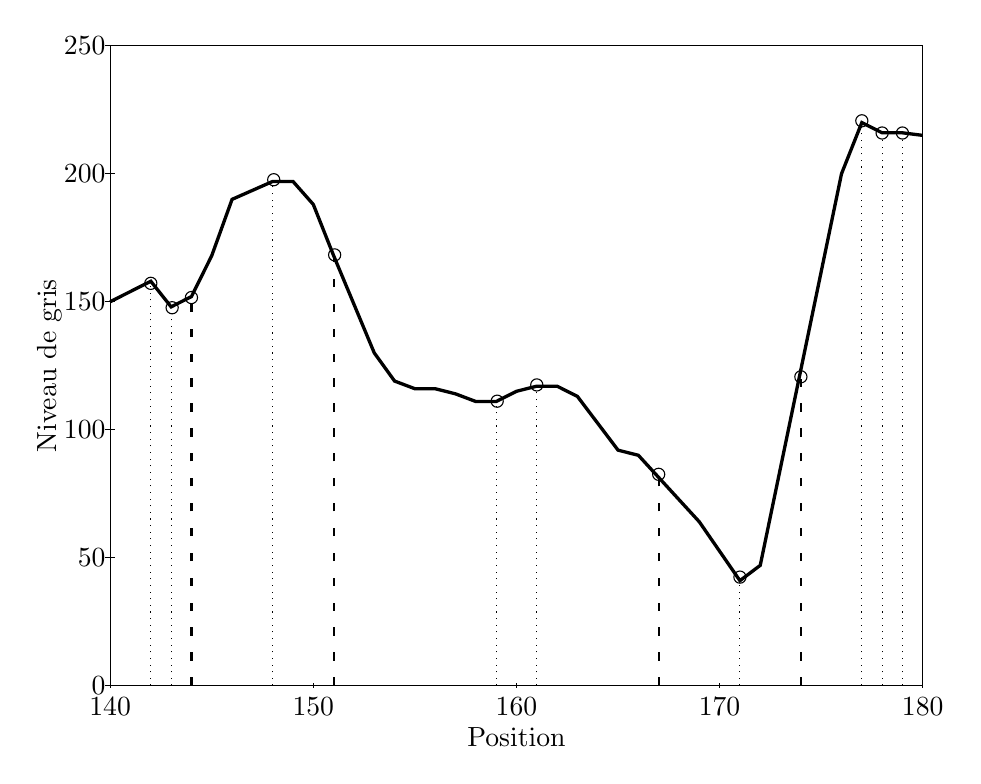
\begin{tikzpicture}[xscale=0.258,yscale=0.0325]
\draw (140,0) rectangle (180,250);
\draw[very thick] (140,150) -- (142,158) -- (143,148) -- (144,152) -- (145,168) -- (146,190) -- (148,197) -- (149,197) -- (150,188) -- (151,168) -- (153,130) -- (154,119) -- (155,116) -- (156,116) -- (157,114) -- (158,111) -- (159,111) -- (160,115) -- (161,117) -- (162,117) -- (163,113) -- (165,92) -- (166,90) -- (169,64) -- (171,41) -- (172,47) -- (176,200) -- (177,220) -- (178,216) -- (179,216) -- (180,215);
\draw[yscale=7.9385] (142,19.8) circle (0.3);
\draw[dotted] (142,0) -- (142,158);
\draw[yscale=7.9385] (143.05,18.6) circle (0.3);
\draw[dotted] (143,0) -- (143,148);
\draw[yscale=7.9385] (144,19.1) circle (0.3);
\draw[loosely dashed,thick] (144,0) -- (144,152);
\draw[yscale=7.9385] (148.05,24.9) circle (0.3);
\draw[dotted] (148,0) -- (148,197);
\draw[yscale=7.9385] (151.05,21.2) circle (0.3);
\draw[loosely dashed,thick] (151,0) -- (151,168);
\draw[yscale=7.9385] (159.05,14) circle (0.3);
\draw[dotted] (159,0) -- (159,111);
\draw[yscale=7.9385] (161,14.8) circle (0.3);
\draw[dotted] (161,0) -- (161,117);
\draw[yscale=7.9385] (167,10.4) circle (0.3);
\draw[loosely dashed,thick] (167,0) -- (167,85);
\draw[yscale=7.9385] (171,5.34) circle (0.3);
\draw[dotted] (171,0) -- (171,41);
\draw[yscale=7.9385] (174,15.2) circle (0.3);
\draw[loosely dashed,thick] (174,0) -- (174,120);
\draw[yscale=7.9385] (177,27.8) circle (0.3);
\draw[dotted] (177,0) -- (177,220);
\draw[yscale=7.9385] (178,27.2) circle (0.3);
\draw[dotted] (178,0) -- (178,216);
\draw[yscale=7.9385] (179,27.2) circle (0.3);
\draw[dotted] (179,0) -- (179,216);

\foreach \x in {140,150,160,170,180} \draw (\x,1) -- (\x,-1) node[anchor=north] {\x};
\foreach \y in {0,50,100,150,200,250} \draw (139.75,\y) -- (140.25,\y) node[anchor=east] {\y};
\node at(160,-20) {Position};
\node[rotate=90] at(137,125) {Niveau de gris};
\end{tikzpicture}
  \caption{Profil d'une ligne d'une image et points utilisés pour la mesure du flou~\cite{marziliano-blurmetric}.}
  \label{fig:marzi}
\end{figure}


\subsubsection{Mesure du \emph{ringing}}
Comme pour le flou, il existe peu de mesures du \emph{ringing}~\cite{feng-spie2006}. Suite à ses travaux sur le flou, Marziliano~\cite{marziliano-ringingmetric} s'y est intéressée, particulièrement dans le cadre de JPEG2000. Sa mesure de \emph{ringing} utilise d'ailleurs celle de flou. En parcourant chaque ligne de l'image, le défaut est mesuré le long de chaque contour. Deux mesures sont alors définies, l'une à gauche du contour, l'autre à droite. Le support total du \emph{ringing} est définit comme la différence entre une largeur constante d'oscillation du \emph{ringing} et la largeur du contour calculée par la mesure de flou. La largeur constante d'oscillation est un a priori sur les effets de la décomposition en ondelettes utilisée dans JPEG2000. La différence entre le minimum et le maximum de l'image de différence est multipliée par la taille de ce support de \emph{ringing}. La mesure de \emph{ringing} du contour est égale à la moyenne entre la valeur de la mesure de gauche et celle de droite. La mesure globale de \emph{ringing} de l'image est calculée en moyennant les mesures locales de tous les contours détectés.

Cette technique souffre évidemment des mêmes défauts que celle de flou. Elle utilise de plus une hypothèse sur la valeur de la largeur d'oscillation spécifique au codage JPEG2000. Cela rend sa mesure extrêmement spécifique à ce système dégradant et en réduit d'autant l'utilisabilité. Elle est cependant l'une des rares mesures de ce défaut.


\subsection{Métriques de qualité}
Certaines études vont plus loin que la mesure de dégradations. À partir d'une ou plusieurs de ces mesures, elles construisent une métrique de qualité. %Nous les classons suivant le nombre de dégradation qu'elles considèrent.


\subsubsection{Métriques basées sur une seule dégradation}
Seule Marziliano a utilisé une unique mesure de dégradations pour prédire la qualité subjective d'images fixes. Elle a évalué les performances de sa mesure de flou par des tests subjectifs réalisés par dix experts avec cinq images fixes originales~\cite{marziliano-blurmetric}. Celles-ci sont dégradées soit synthétiquement par un filtre gaussien, soit par un codeur JPEG2000. Cinq dégradations de chaque type sont appliqués sur chaque image. Le coefficient de corrélation entre les notes subjectives et les mesures calculées est de 0,96 pour les images dégradées par le filtrage gaussien et de 0,85 pour les images dégradées par JPEG2000. Les bonnes performances avec le filtre gaussien ne sont pas surprenantes car la mesure y est bien adapté, de par son principe. La faible valeur obtenue avec JPEG2000 s'explique par le fait que cette compression n'engendre pas seulement du flou mais aussi d'autres dégradations, dont du \emph{ringing}.

Elle évalue également sa métrique de \emph{ringing}~\cite{marziliano-ringingmetric}. Des tests subjectifs sont réalisés avec neuf images originales et cinq qualités JPEG2000. Le coefficient de corrélation entre les mesures subjectives et les notes objectives est de 0,85. L'auteur explique cette faible valeur par le fait qu'il est difficile pour les observateurs d'évaluer le \emph{ringing} seul dans les images JPEG2000. Ceci montre la difficulté de réaliser des tests psychophysiques demandant aux observateurs de ne se focaliser que sur un unique type de dégradations alors que d'autres sont simultanément présents.


\subsubsection{Métriques basées sur plusieurs dégradations}
Baser une métrique de qualité sur plusieurs mesures de dégradations pose le problème de leur cumul. Les modèles utilisés par la majorité des métriques sont souvent simples. Par exemple, Wang combine une mesure de flou et une d'effet de bloc~\cite{wang-icip2002}. Ces deux mesures sont issues de sa mesure d'effet de bloc~\cite{wang-icip2000}. Le flou est alors estimé par le décalage d'énergie des hautes fréquences vers les basses fréquences. Trois caractéristiques sont calculées avant de générer la note de qualité finale. Chacune est mesurée verticalement et horizontalement, la moyenne des deux mesures étant considérée dans la suite. La première caractéristique est la mesure de l'effet de bloc $b_W$. La seconde est dérivée de la mesure de flou et de celle d'effet de bloc, les auteurs la nomment mesure d'activité $a_W$. La dernière est issue du calcul des gradients vertical et horizontal. Les compteurs $z_h$ et $z_v$ sont incrémentés à chaque fois que les gradients horizontal et vertical s'annulent respectivement. La caractéristique $z_W$ est égale à la moyenne de ces compteurs divisée par le nombre de valeurs du gradient. Enfin, la note de qualité est donnée par le modèle :
\begin{equation}
M_W = \alpha + \beta\cdot b_W^{\gamma_1}\cdot a_W^{\gamma_2}\cdot z_W^{\gamma_3}
\end{equation}
%
avec $\alpha$, $\beta$, $\gamma_1$, $\gamma_2$ et $\gamma_3$ les paramètres à optimiser. Cette optimisation est obtenue à partir de données subjectives, c'est-à-dire que les valeurs retenues sont celles minimisant l'erreur de prédiction de MOS connus. Le danger de ce type d'approche est le sur-entrainement du modèle. Si les données manquent de variété, par exemple dans la gamme d'activité des images, les paramètres ne s'adapteront pas à des conditions différentes et le modèle manquera de robustesse.

Farias~\cite{farias-phd} propose un critère de qualité intégrant à la fois une mesure d'effet de bloc $b_F$, une de flou $f_F$ et une de bruit $n_F$. Les mesures utilisées sont adaptées de mesures existantes dans la littérature comme celle de Vlachos~\cite{vlachos-detection} pour l'effet de bloc et celle de Marziliano~\cite{marziliano-blurmetric, marziliano-ringingmetric} pour le flou. Le modèle de cumul final utilise une sommation de Minkowski :
\begin{equation}
M_F = \left( w_b\cdot b_F^p + w_f\cdot f_F^p + w_n\cdot n_F^p \right)^{\frac{1}{p}}
\end{equation}
%
avec $\beta$ l'exposant de la sommation et $w_b$, $w_f$ et $w_n$ les pondérations des mesures $b_F$, $f_F$ et $n_F$ respectivement. Ces pondérations peuvent être nulles, si l'une ou plusieurs des mesures ne sont pas prises en compte. Le cumul adopté est donc très simple. Cela est regrettable compte tenu de la nature de l'étude. Elle consistait en effet à mesurer à la fois la gêne induite par chaque dégradation, par leurs combinaisons et par un système dégradant de type MPEG-2. Cela aurait pu mener à un modèle de cumul plus évolué car bâtit sur des résultats psychovisuels individuels, combinés et comparés à des dégradations réelles.

Caviedes~\cite{caviedes-nrqm} a une approche similaire mais en plus de mesures de dégradations liées au codage, il intègre des mesures de contraste et de netteté. Au final, il combine six mesures : $b_C$ pour l'effet de bloc ; $r_C$ pour le \emph{ringing} ; $c_C$ pour le \emph{clipping}, dégradation due à la troncation de bits imposée par la précision des calculs ; $n_C$ pour le bruit ; $o_C$ pour le contraste et enfin $s_C$ pour la netteté. La méthode de détermination du cumul est la suivante. Les auteurs disposent d'un ensemble de séquences d'entrainement, dont ils connaissent les mesures subjectives et les six notes objectives. Plutôt que de chercher une solution de manière exhaustive, les auteurs adoptent une approche incrémentale. Les mesures sont ajoutées et évaluées au fur et à mesure. Cela permet à la fois de limiter les calculs mais aussi d'évaluer l'apport de chaque contribution en termes d'impact sur la qualité subjective. Dans un premier temps, les six mesures principales sont calculées. La seconde étape fournit les interactions entre certaines de ces mesures. Finalement, la mesure de qualité NROQM \emph{(No-reference objective quality metric)} est obtenue par la formule :
\begin{equation}
\begin{array}{rl}
M_C =	& - \frac{1}{\gamma_3}\left(1+o_C + \frac{n_C}{\gamma_1}\right)\left( b_C^{\gamma_2} + \frac{b_C}{1+b_C}r_C^{\gamma_2} \right) - (1+ o_C)(1+\gamma_4\times c_C)^{\gamma_5}\\
			& - \gamma_6n_Cs_Co_C - \frac{1}{\left( 1+\gamma_4c_C\right)^{\gamma_7}}\left( \frac{n_C}{o_C}\right)^{\gamma_8} - \left( \gamma_9+\gamma_{10}o_C\right)^{\gamma_{11}} + s_C
\end{array}
\end{equation}
%
avec $\gamma_i ; i \in [1 ; 11]$ les paramètres du modèle. Plus évolué, celui-ci montre bien la complexité à laquelle le cumul de différentes mesures peut mener. L'approche incrémentale adoptée est originale. Elle permet de ne pas considérer toutes les mesures en un bloc, mais de les ajouter au modèle une par une. La question qui se pose néanmoins est de savoir si l'ordre adopté pour ajouter ces mesures a une influence sur le modèle de cumul obtenu.


\section{Discussion}
\subsection{Sur la diversité des approches}
Dans ce chapitre, nous avons présenté quelques critères de qualité afin d'appréhender les diverses approches existant dans la littérature. Ce panorama montre la richesse et le dynamisme du domaine de l'évaluation objective de la qualité de l'image et de la vidéo. Cela n'est pas surprenant devant l'importance actuelle de ces médias numériques.

L'approche purement signal est la plus utilisée par le domaine du codage alors que c'est celle qui propose le moins de critères. Pourtant, nous pouvons nous interroger sur la prise de conscience de ses limites et de son bon usage. Lorsque la demande en robustesse s'accroit, les utilisateurs de critères de qualité sont alors demandeurs de critères précis, robustes et si possible, capables d'évaluer une séquence en temps-réel. Reconnaissons tout de même que peu de critères existants remplissent ces conditions.

Les critères basés sur la modélisation bas niveau du système visuel humain sont intéressants car ils sont proches du phénomène réel de la vision humaine. Cette proximité leur permet d'être génériques, car ils ne dépendent ni d'un système dégradant, ni d'un système d'affichage, ni d'un mode de transmission. Les études engagées dans cette voie permettent parallèlement d'acquérir une connaissance accrue sur le mode de fonctionnement bas niveau de l'observateur humain. Les applications de telles connaissances sont larges et vont bien au-delà de l'évaluation de la qualité d'image ou de la vidéo. Cependant dans le contexte de l'évaluation de la qualité vidéo, la modélisation des phénomènes bas niveau ne suffit pas. L'absence de prise en compte des aspects haut niveau restreint fortement les performances. De plus, ces critères sont souvent complexes à mettre en \oe uvre et à expliquer aux ingénieurs désireux d'en appréhender l'usage.

Les approches basées sur la fidélité structurelle permettent de considérer certains aspects de plus haut niveau. La simplicité des calculs mis en jeu facilite le traitement, l'analyse et l'optimisation des algorithmes. Cependant, le paradigme structurel de l'image, tel qu'il est posé en hypothèse, est discutable. Aucune définition de cette structure n'est usuellement admise. Rien n'assure que les dégradations de la structure mesurées par ces critères correspondent à une réalité perceptuelle.

Enfin, les approches basées sur la mesure explicite de dégradations haut niveau sont étroitement liés aux systèmes dégradants existants. La principale limite de l'approche vient de la difficulté d'isoler les effets d'une dégradation donnée. Une liste de dégradations ne correspond pas à des effets isolés appliqués successivement, mais à un processus complexe où les dégradations se superposent les unes aux autres dans l'espace et dans le temps. Cette technique rend également délicate l'évaluation subjective des dégradations, car il est difficile pour l'observateur de les isoler.


\subsection{Sur les performances}
Nous l'avons vu, il difficile de comparer une telle diversité d'approches ou même certains critères existants. VQEG est le groupe d'experts chargé de cette tâche. En plus de 10 ans d'existence, il a publié deux études comparatives sur les critères d'évaluation de la télévision avec référence complète~\cite{vqeg-frtv1,vqeg-frtv2}. Les travaux actuels portent sur l'évaluation de la télévision avec référence réduite ou sans référence, du multimédia et de la télévision haute définition. Le plan de tests portant sur le multimédia~\cite{vqeg-MMtestplan} est sur le point d'être achevé. Pour comprendre le considérable effort que cela représente, signalons que ce plan prévoit l'étude avec trois résolutions d'affichage, 14 tests par résolutions et 136 vidéos par test. Ces tests sont réalisés par de nombreux laboratoires de par le monde, pour un total dépassant 5000 vidéos évaluées.

La première campagne a notamment montré que les critères basés sur la modélisation bas niveau du système visuel humain n'obtiennent pas de performances significativement supérieures à celles du PSNR. Lors de la seconde campagne d'évaluation, deux tests distincts ont été réalisés. Le premier utilisait des séquences au format PAL de 625 lignes, le second des séquences au format NTSC de 525 lignes. Les résultats de l'étude sur les deux tests sont proches, sans être cependant identiques. En général, les critères obtiennent des performances différentes sur les deux tests. Le meilleur coefficient de corrélation, obtenu par VQM~\cite{wolf-vqmtech}, est de 0,938 sur les séquences NTSC. Le même critère n'obtient plus que 0,886 sur l'autre test. Métrique un peu particulière car combinant des aspects signal et perceptuel, VQM sera plus particulièrement détaillée dans le chapitre suivant. La différence de performance est sensible, alors que les deux jeux de séquences ne sont pas très différents. Il semble donc difficile de réaliser un critère robuste qui fonctionnerait bien dans des configurations différentes. La quête du critère unique à usage multiple est semble-t-il vaine, tant la diversité des conditions d'utilisation est grande.

Les approches basées sur la mesure explicite de dégradations haut niveau obtiennent de bonnes performances sur des images dégradées synthétiquement. Cependant, ces performances chutent fortement dans des conditions réelles de codage. Ainsi, les utiliser individuellement pour considérer la qualité n'est pas envisageable. En combiner plusieurs soulève le problème de leur combinaison. %En outre, considérer une liste de dégradations haut niveau ne permet pas d'atteindre l'origine réelle de toutes ces dégradations : l'erreur de quantification.


\subsection{Sur les cumuls}
Tout critère se trouve confronté au problème du cumul des grandeurs locales en une note de qualité finale. Pourtant, nous avons constaté que cet aspect était rarement approfondi par les critères de qualité d'image et de vidéo. Ce cumul est souvent réduit à une sommation de Minkowski qui ne prend pas en compte tous les aspects des grandeurs à fusionner. Or, nous considérons qu'il revêt une grande importance dans la structure globale d'un critère de qualité. En effet, il correspond à l'élaboration finale de la note de qualité. C'est là que l'observateur fusionne l'ensemble des erreurs qu'il a perçu en une évaluation quantitative de la qualité de la séquence.

Nous distinguons trois intégrations majeures : sur les grandeurs locales, sur l'espace et sur le temps. Suivant l'approche adoptée, la nature des grandeurs locales varie. Si le critère décompose la vidéo en composantes perceptuelles, il faudra fusionner les fréquences. S'il utilise des caractéristiques calculés dans des blocs, il faudra fusionner ces caractéristiques. La figure~\ref{fig:figCumul} présente un exemple d'enchainement de ces intégrations.

\begin{figure}[htbp]
	\centering
	\begin{tikzpicture}[text centered, node distance = 3cm]% \begin{tikzpicture}[text centered]
% Place nodes
	\node[text width=2cm] (info) {grandeurs locales};
	\node[action, right of=info, text width=2cm] (cumul) {cumul sur les grandeurs};
	\node[action, right of=cumul] (spatial) {cumul spatial};
	\node[action, right of=spatial,text width=2cm] (temp) {cumul temporel};
	\node[right of=temp] (note) {note finale};

% Draw edges
	\path[fleche] (info) -- (cumul);
	\path[fleche] (cumul) -- (spatial);
	\path[fleche] (spatial) -- (temp);
	\path[fleche] (temp) -- (note);
% \end{tikzpicture}\end{tikzpicture}
	\caption{Exemple d'enchainement des cumuls à effectuer pour fusionner les grandeurs locales en une note de qualité finale.}
	\label{fig:figCumul}
\end{figure}

L'ordre utilisé sur cette figure n'est qu'un exemple. En fait, la manière dont les différents cumuls s'enchainent est une question à laquelle peu de travaux se sont intéressés. Citons le cas du cumul fréquentiel, pour lequel Bekkat~\cite{bekkat-phd} a montré que l'ordre entre le cumul angulaire et le cumul radial n'était pas un élément sensible. D'après Le Callet~\cite{lecallet-phd}, il faut systématiquement effectuer le cumul fréquentiel avant le cumul spatial car cet ordre traduit la stratégie du système visuel humain à percevoir les dégradations d’abord localement, puis à regrouper l’ensemble des dégradations perçues sur tous les sites de l’image.

Au final, la méthode de cumul idéale n'est pas encore bien connue. Mettant en jeu des comportements haut niveau du système visuel humain, la construction du jugement à partir de mesures locales nécessite encore un approfondissement certain. En particulier, le passage de l'évaluation de qualité de l'image à celle de la vidéo est un point sensible du problème, spécifique aux critères de qualité vidéo. En effet, utiliser un critère pour image fixe et considérer que la mesure de qualité de la séquence est la moyenne des mesures de qualité des images de la séquence est particulièrement inefficace. Les interactions espace-temps ont donc un impact non négligeable dans la construction du jugement. Pourtant, il existe encore peu d'études sur ce point précis dans la littérature.


\section{Conclusion}
Dans ce chapitre, nous avons réalisé une vue d'ensemble des approches existantes en termes de critères objectifs de la qualité vidéo. Nous avons classé les grands courants de recherche actuels en quatre familles principales : l'approche purement signal ; les approches basées sur la modélisation de la vision humaine bas niveau ; les approches basées sur la fidélité structurelle ; les approches basées sur la mesure explicite de dégradations haut niveau.

L'approche purement signal consiste à utiliser des outils basiques considérant les différences pixel à pixel entre séquences. Bien que très répandues et utilisables dans des conditions particulières, ces métriques ne sont pas assez robustes dans leur prédiction de la qualité vidéo. Les approches basées sur la modélisation de la vision humaine bas niveau sont plus évoluées et plus complexes. Malgré leur capacité à mesurer des phénomènes locaux, elles ne prennent assez en considération les aspects haut niveau du système visuel humain pour réussir à en reproduire fidèlement le comportement. Tentant de prendre en compte certains de ces aspects haut niveau, les approches basées sur la fidélité structurelle ont montré de bonnes performances sur certains ensembles de séquences. Cependant, les métriques proposées ont l'inconvénient de générer une prédiction très sensible aux facteurs intervenant dans leur calcul. De plus, la définition même de la structure d'une image ou d'une vidéo reste à établir clairement. Enfin, les approches basées sur la mesure explicite de dégradations haut niveau considèrent les impacts du codage tels que l'effet de bloc ou le flou. Cependant, mesurer ces effets individuellement n'a pas beaucoup de sens dans la mesure où le codage est un phénomène complexe où les dégradations sont inter-dépendantes. Les individualiser est une approche périlleuse, autant pour leur notation objective que pour leur évaluation subjective. Les travaux de Farias~\cite{farias-phd} ont de plus montré que cette approche n'est pas toujours robuste sur des contenus différents.

Les multiples approches proposées n'ont donc pas apporté, loin s'en faut, toutes les solutions à la problématique de l'évaluation objective de la qualité. Notamment, la problématique du cumul des grandeurs locales en une note de qualité finale n'est pas encore bien caractérisée et souvent sous-estimée. De plus, le cadre spécifique de la télévision haute définition, dont nous avons montré les différences significatives avec la télévision standard, n'est pas traité. VQEG prépare actuellement son plan de test adapté à ce contexte~\cite{vqeg-hdtvtestplan}. Comment les métriques existantes s'y comporterait-elles ? C'est l'une des questions auxquelles le chapitre suivant tente d'apporter une réponse.


\ornementChapitre
